\section{Results}
To test the distortion and directionality of the directional speaker, recordings were made where a 2.5 kHz tone was generated, appropriately pre-processed using julia and produced into the testing environment by the ultrasonic directional speaker. The distortion was compared to a classical loudspeaker and the same ultrasonic directional speaker but without the pre-processing provided by the julia code. The directivity testing was achieved by sweeping the transducer array and classical loudspeaker across the microphone at a distance of 1.75m. The arc transitioned the speaker faces between -90$^\circ$ to +90$^\circ$ relative to the microphone. Following these tests, the recordings were imported into julia where they were processed with appropriate filtering and transformation to demonstrate the directionality and distortion of the ultrasonic directional speaker.
\subsection{Distortion testing}
The distortion testing of the square root AM system is expected to produce a fundamental signal at 2.5kHz with decreasing magnitudes for 1st and 2nd harmonics at 5kHz and 7.5khz respectively. The same tests without the square root pre-processing applied should produce larger magnitude harmonics while the traditional loudspeaker should produce little to no harmonics.
\subsubsection{Traditional loudspeaker distortion results}

\begin{figure}[ht!]
    \centering
    \begin{minipage}{0.49\textwidth}
        \centering
        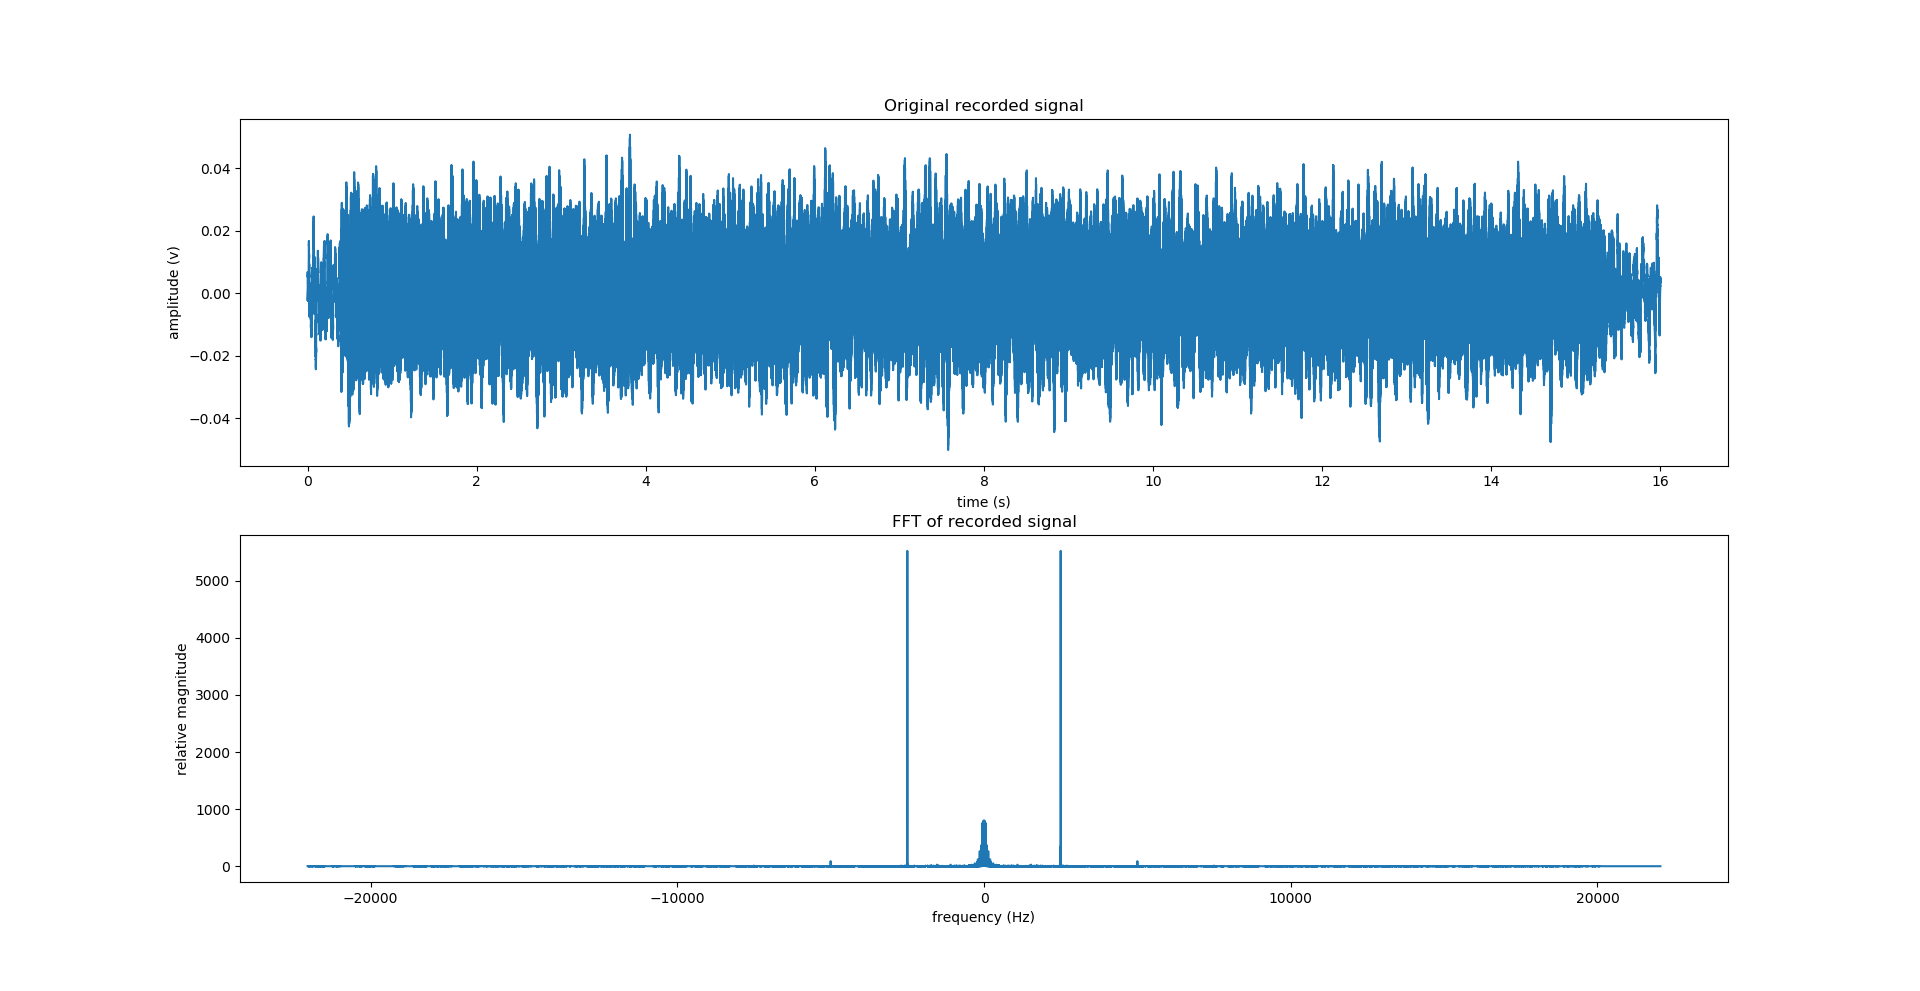
\includegraphics[width=\textwidth]{Figures/Testing/Distortion/Spk_fft_sig.png}
        \caption{The spectrum and time domain signal of the traditional loudspeaker with a 2.5kHz input tone}
        \label{fig:spk_fft_dist}
    \end{minipage}\hfill
    \begin{minipage}{0.49\textwidth}
        \centering
        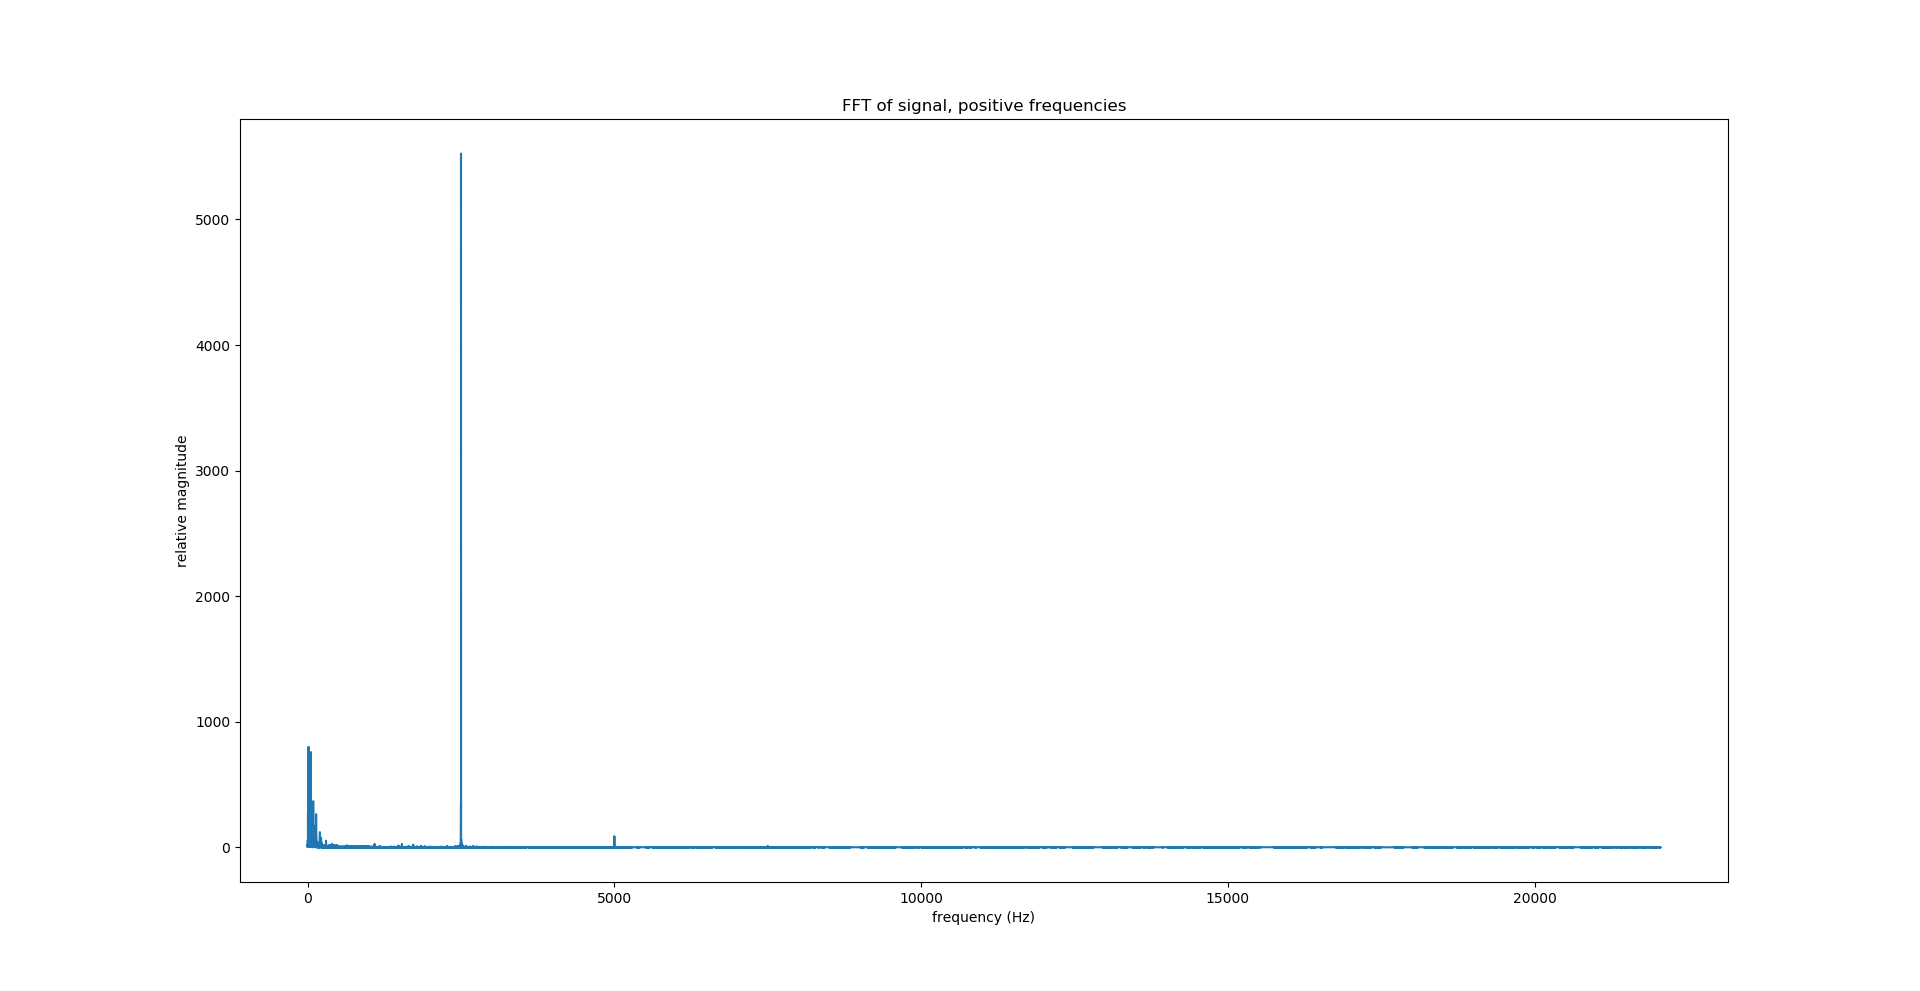
\includegraphics[width=\textwidth]{Figures/Testing/Distortion/Spk_fft_pos.png}
        \caption{The positive spectrum of the traditional loudspeaker with a 2.5kHz input tone}
        \label{fig:spk_fft_dist_pos}
    \end{minipage}
\end{figure}

The results in figure \ref{fig:spk_fft_dist} and \ref{fig:spk_fft_dist_pos} indicate a strong presence of the 2.5kHz test tone with some smaller low frequency noise likely caused by background noise as well as a small 1st harmonic at 5kHz.

\newpage
\subsubsection{Square-root AM versus AM ultrasonic directional speaker distortion results}
\begin{figure}[ht!]
    \centering
    \begin{minipage}{0.49\textwidth}
        \centering
        
            \centering
            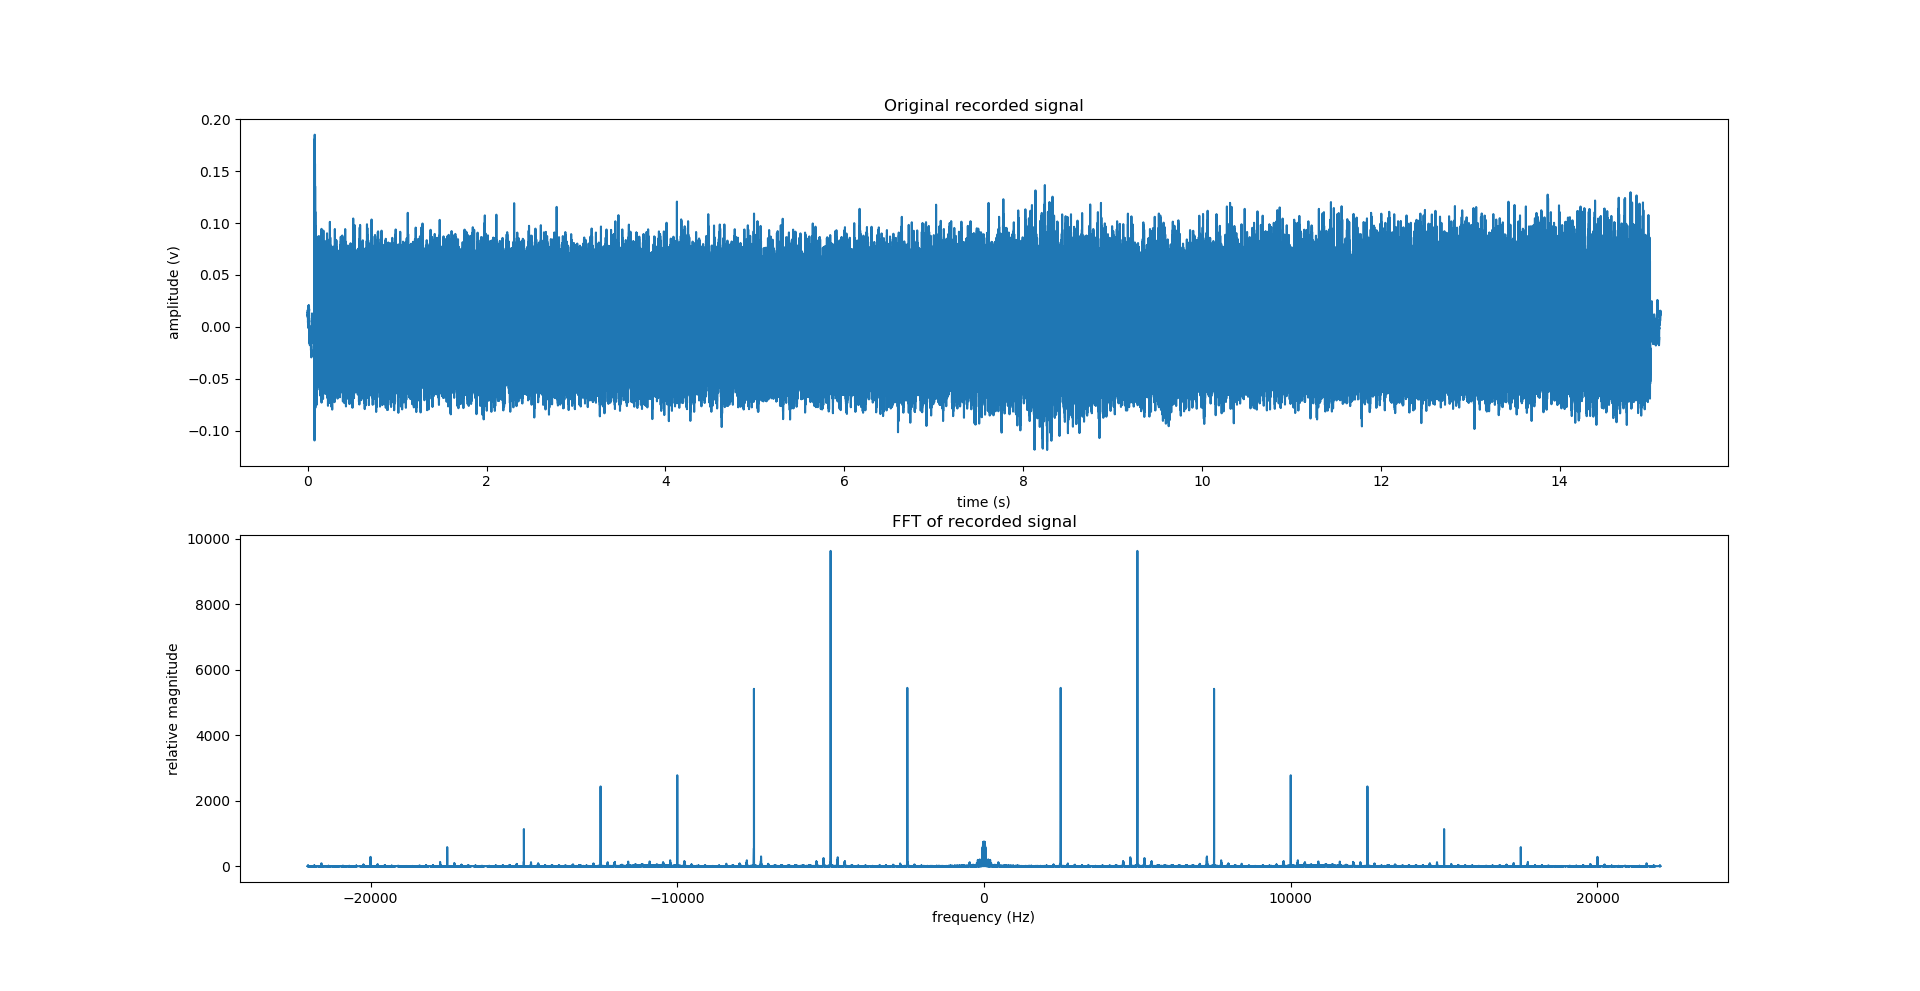
\includegraphics[width=\textwidth]{Figures/Testing/Distortion/SQRT_fft_sig_straighton.png}
            \caption{The spectrum and time domain signal of the square root amplitude modulated ultrasonic speaker with a 2.5kHz input tone}
            \label{fig:sqrt_fft_dist}
        
        
            \centering
            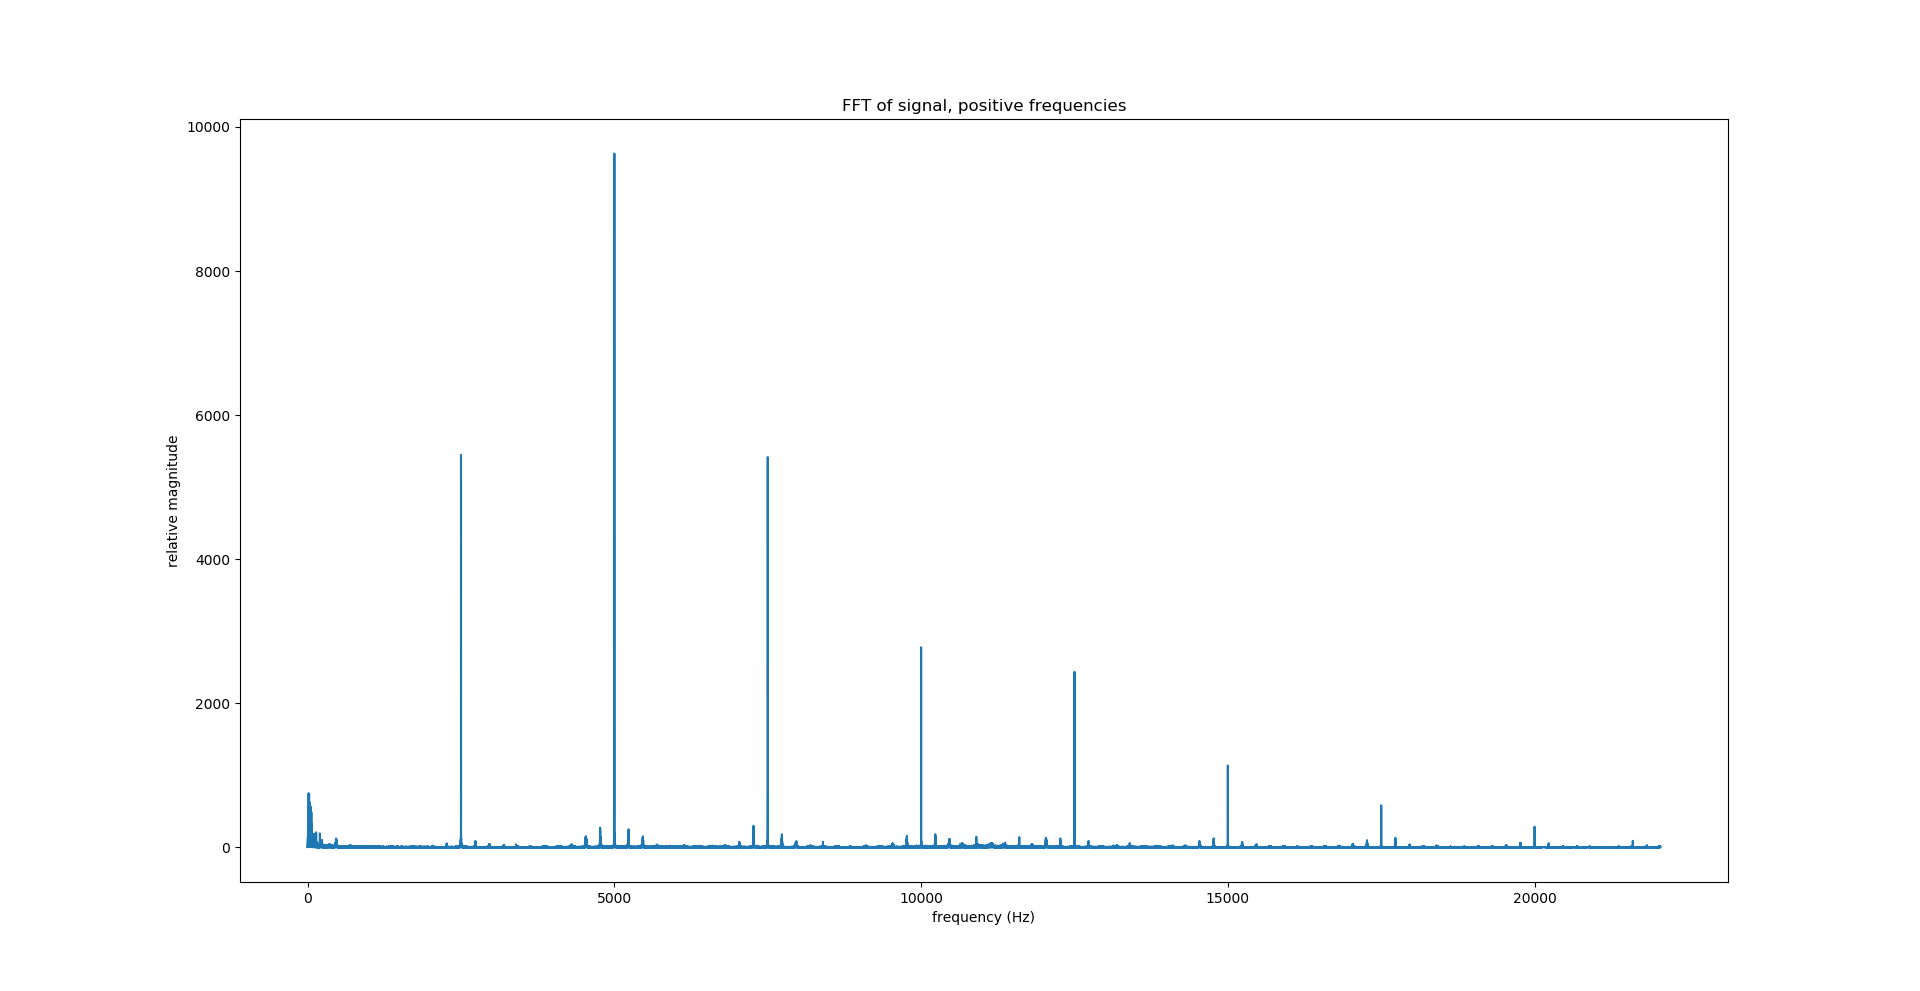
\includegraphics[width=\textwidth]{Figures/Testing/Distortion/SQRT_fft_pos_straighton.png}
            \caption{The positive spectrum of the square root amplitude modulated ultrasonic speaker with a 2.5kHz input tone}
            \label{fig:sqrt_fft_dist_pos}
        
    \end{minipage}\hfill
    \begin{minipage}{0.49\textwidth}
        \centering
        
            \centering
            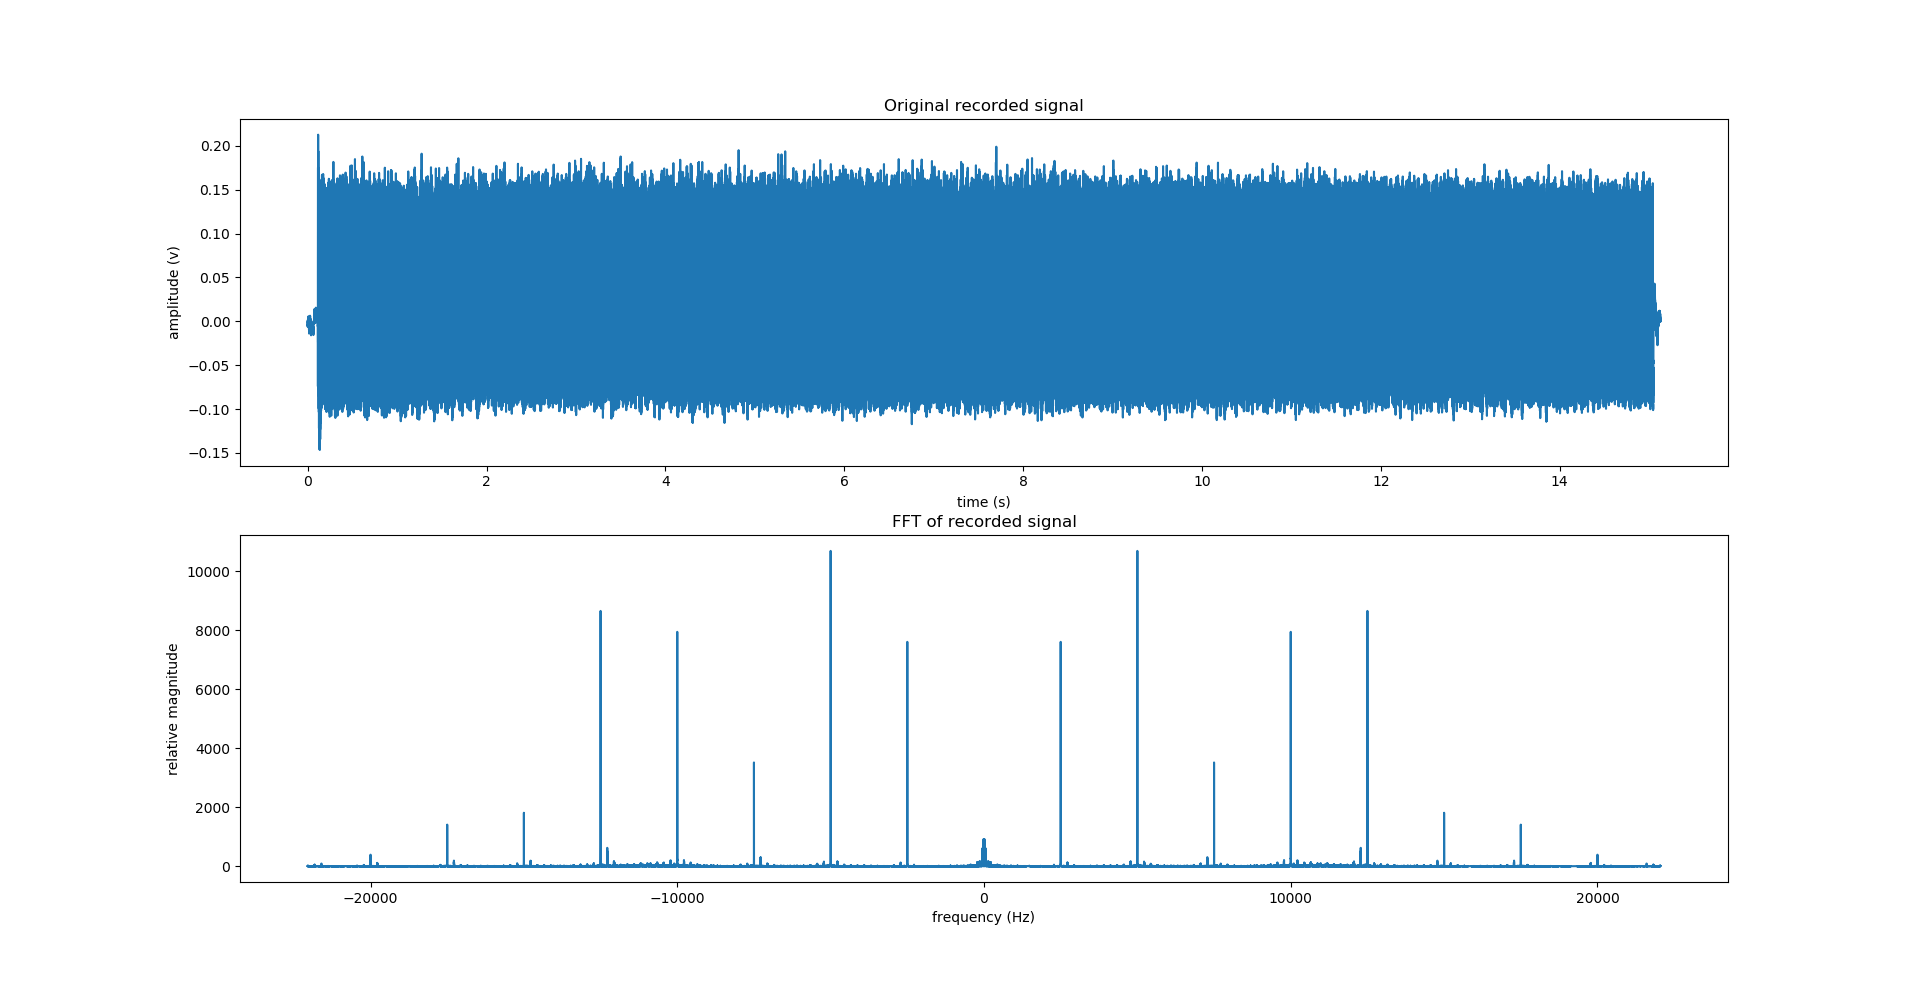
\includegraphics[width=\textwidth]{Figures/Testing/Distortion/AM_fft_sig.png}
            \caption{The spectrum and time domain signal of the amplitude modulated ultrasonic speaker with a 2.5kHz input tone}
            \label{fig:AM_fft_dist}
        
        
            \centering
            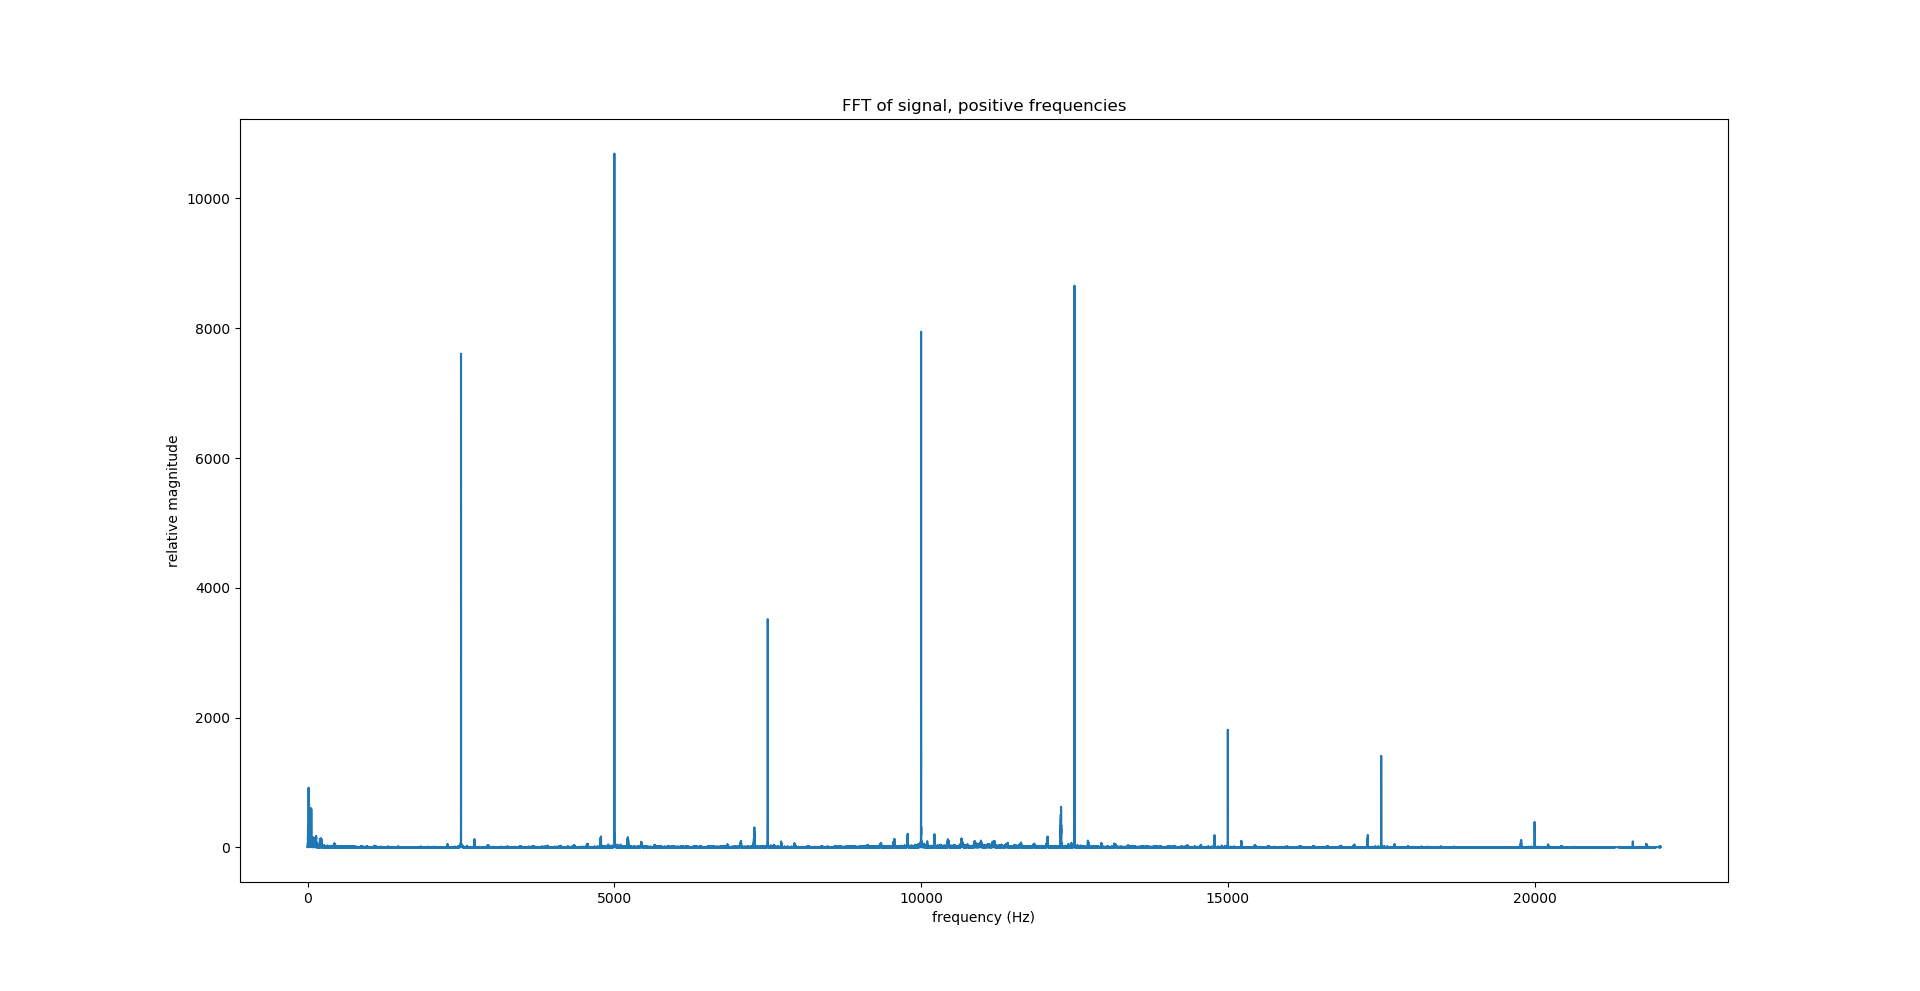
\includegraphics[width=\textwidth]{Figures/Testing/Distortion/AM_fft_pos.png}
            \caption{The positive spectrum of the amplitude modulated ultrasonic speaker with a 2.5kHz input tone}
            \label{fig:AM_fft_dist_pos}
        
    \end{minipage}
\end{figure}

%\begin{figure}
%    \centering
%    \begin{minipage}{0.4\textwidth}
%        \centering
%    
%    \end{minipage}\hfill
%    \begin{minipage}{0.4\textwidth}
%        \centering
%    
%    \end{minipage}
%\end{figure}
The results in figure \ref{fig:sqrt_fft_dist} and \ref{fig:sqrt_fft_dist_pos} for the ultrasonic directional speaker with square root pre-processing show a strong tone at the 1st harmonic of the test tone (5kHz). This result appeared only when the microphone was placed into the ultrasonic beam as figures  \ref{fig:sqrt_fft_dist_outofbeam} and \ref{fig:sqrt_fft_dist_pos_outofbeam} show the results for the ultrasonic beam being directed away from the microphone. The signal levels are lower than the original result but the fundamental frequency now lies on 2.5kHz.\\

The results of the ultrasonic directional speaker without any pre-processing are presented in figures \ref{fig:AM_fft_dist} and \ref{fig:AM_fft_dist_pos}. Comparing the spectrum of the speaker to the square root AM system in figures \ref{fig:sqrt_fft_dist} and \ref{fig:sqrt_fft_dist_pos}, the harmonics appear to be even more pronounced and amplified when no pre-processing is applied. Figure \ref{fig:AM_fft_dist_pos} indicates the 1st harmonic to be the largest, followed by the 4th harmonic, then 3rd and finally the fundamental. Additionally, the magnitudes of these harmonics are larger than the square root AM tests.
\begin{figure}[ht!]
    \centering
    \begin{minipage}{0.49\textwidth}
        \centering
        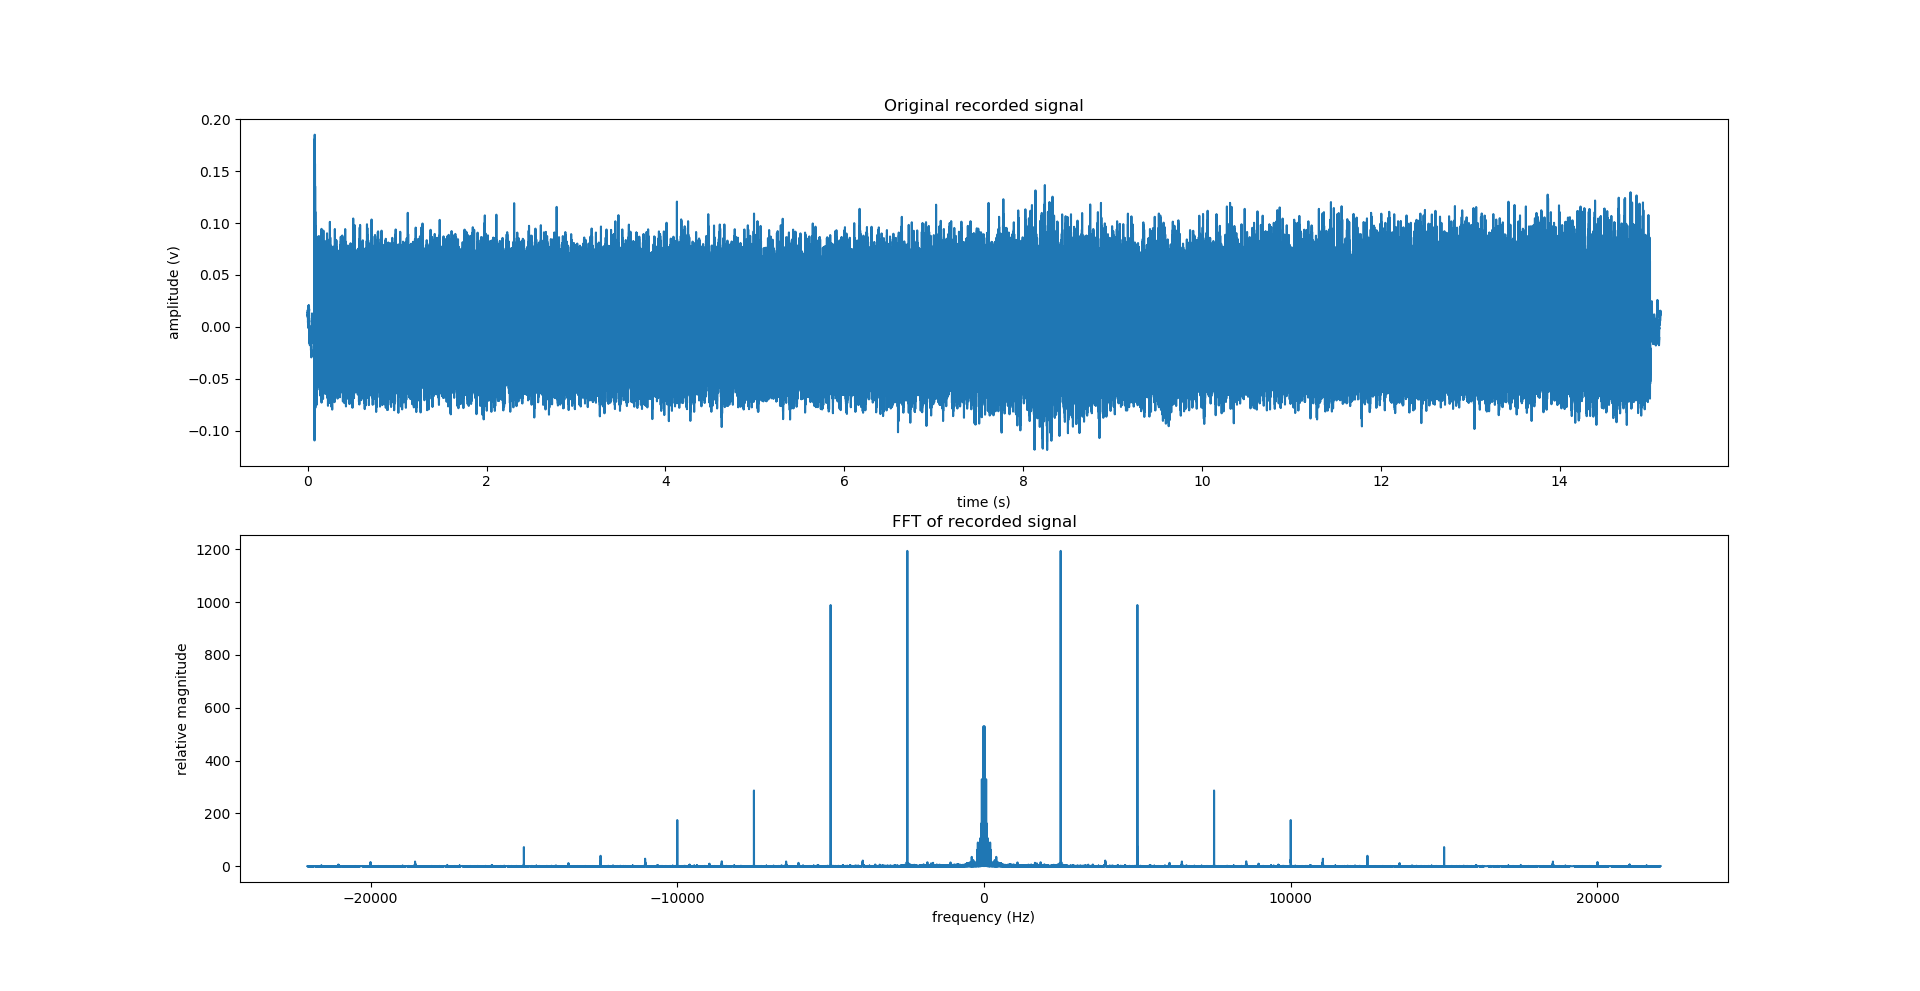
\includegraphics[width=\textwidth]{Figures/Testing/Distortion/SQRT_fft_sig.png}
        \caption{The spectrum and time domain signal of the square root amplitude modulated ultrasonic speaker (microphone outside of beam) with a 2.5kHz input tone}
        \label{fig:sqrt_fft_dist_outofbeam}
    \end{minipage}\hfill
    \begin{minipage}{0.49\textwidth}
        \centering
        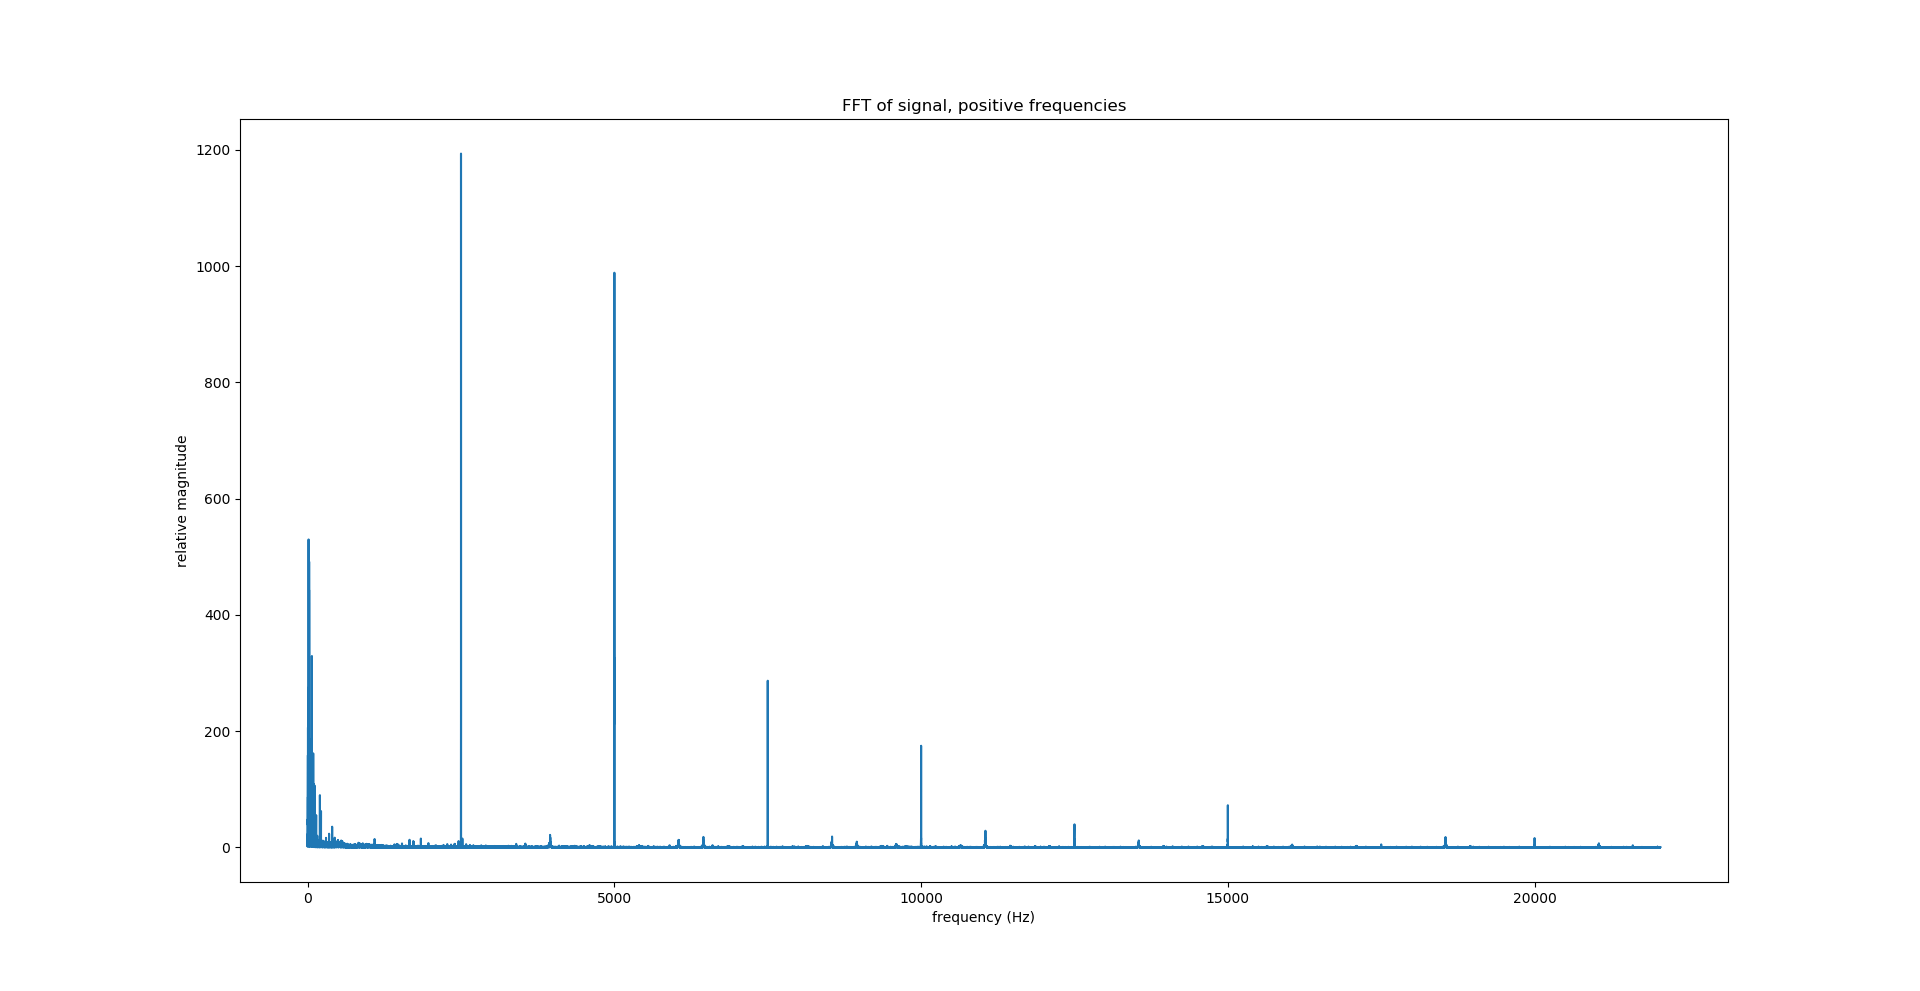
\includegraphics[width=\textwidth]{Figures/Testing/Distortion/SQRT_fft_pos.png}
        \caption{The positive spectrum of the square root amplitude modulated ultrasonic speaker (microphone outside of beam) with a 2.5kHz input tone}
        \label{fig:sqrt_fft_dist_pos_outofbeam}
    \end{minipage}
\end{figure}

\subsection{Directivity testing}
The test setup for directivity testing involved sweeping the transducer/speaker in an arc such that the center of the radiated beam sweeps from left to right of the microphone while producing a tone. The recordings were then cut to the length of the sweep and filtered to demonstrate the signal level of the fundamental 2.5kHz tone as well as its 1st and 2nd harmonics at 5 and 7.5 kHz respectively.

\subsubsection{Directivity of a traditional loudspeaker}
The unfiltered recording of the loudspeaker beam sweep is analysed in figure \ref{fig:unfiltered_spkr_beamsweep} where the time and frequency domain representations of the signal are presented for the loudspeaker beam sweep.
\begin{figure}[ht!]
    \centering
    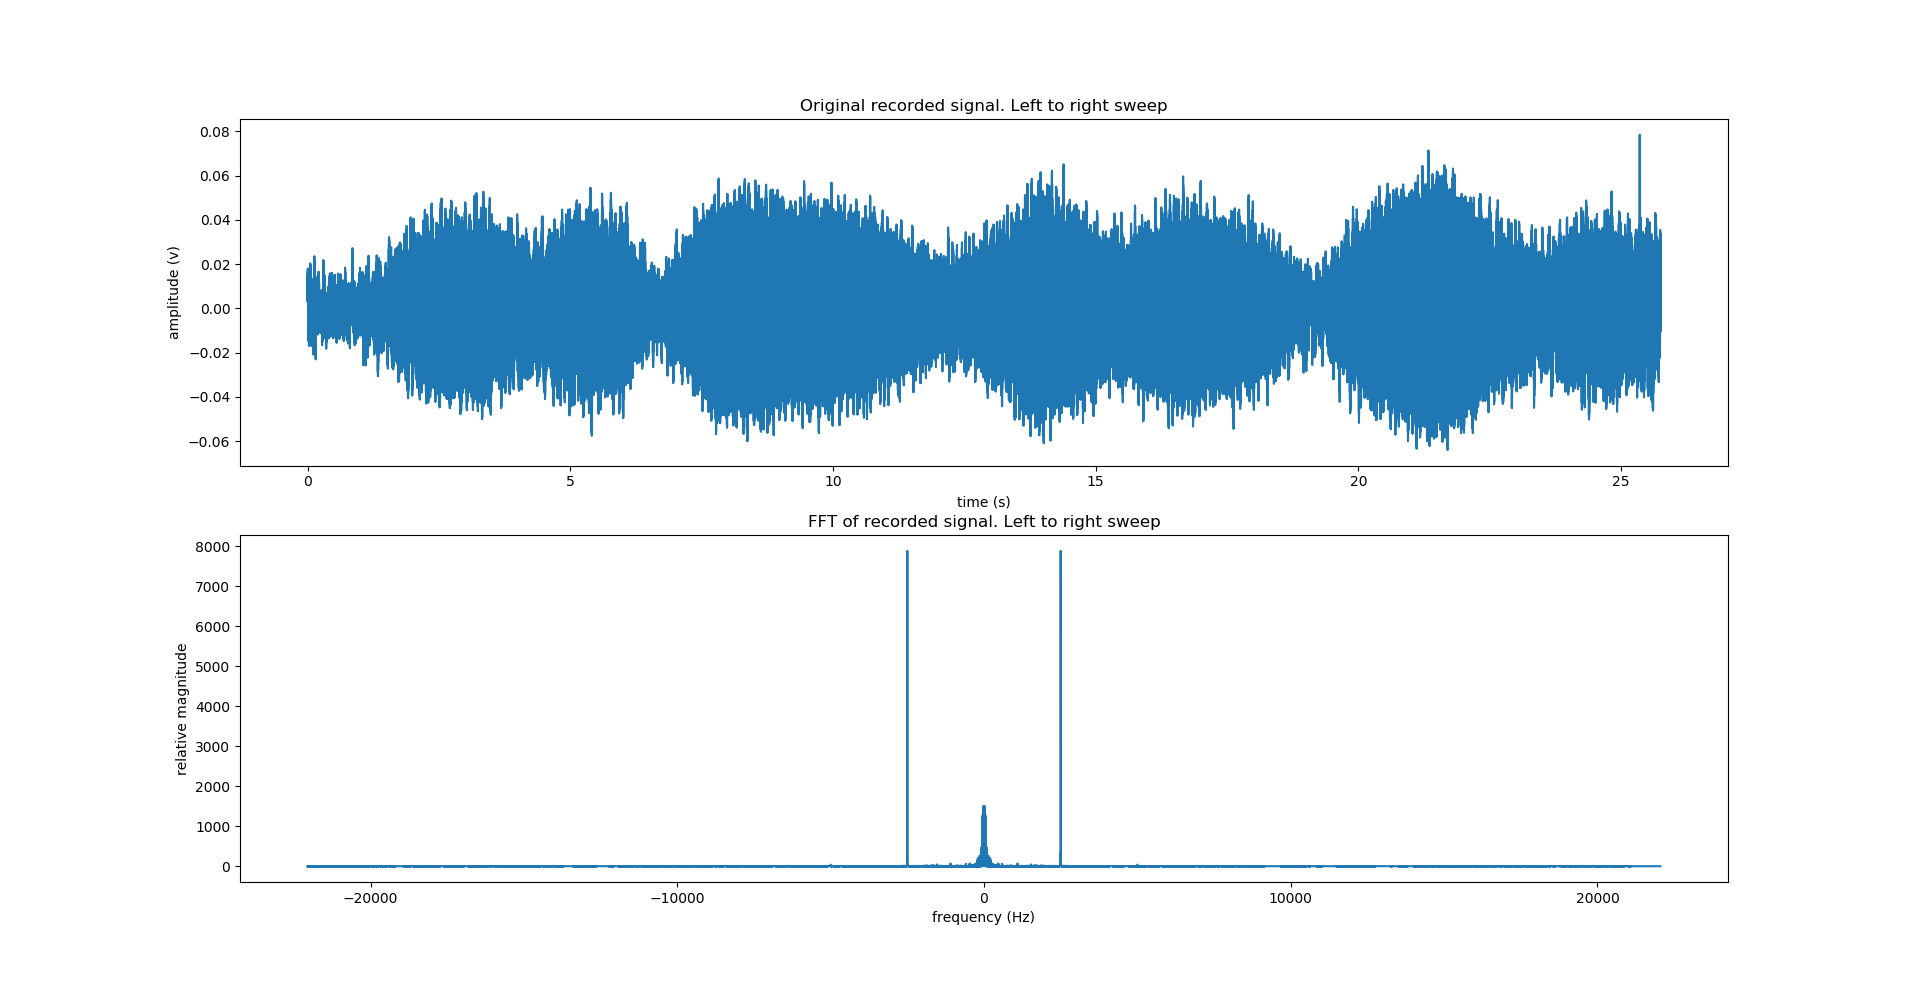
\includegraphics[width=0.8\textwidth]{Figures/Testing/BeamSweep/Classical_speaker/original_sig_fft_amp_skpr.png}
    \caption{Original beam sweep recording and FFT of all samples for traditional loudspeaker}
    \label{fig:unfiltered_spkr_beamsweep}
\end{figure}

\paragraph{Filtered 2.5 kHz beam sweep results}
Figures \ref{fig:spkr_sweep25k_amp} and \ref{fig:spkr_sweep25k_spectro} show the time and frequency domain representations of the recorded beam sweep for a traditional loud speaker. Figure \ref{fig:spkr_sweep25k_amp} demonstrates a mostly consistent volume for the duration of the entire beam sweep, oscillating between approximately $\pm$0.04 V with the smallest troughs at around 7 and 19 seconds. The maximum peaks occur at approximately 9 and 22 seconds which are just after the aforementioned troughs. The results represent a signal without significant directionality as similar sound pressure levels and thus, recorded amplitudes are measured throughout the beam sweep.The spectrogram in figure \ref{fig:spkr_sweep25k_spectro} demonstrates what portion of the spectrum was used to create the time domain signal in figure \ref{fig:spkr_sweep25k_amp} but doesn't show significant variation in signal magnitude over the sweep.
\begin{figure}[ht!]
    \centering
    \begin{minipage}{0.49\textwidth}
        \centering
        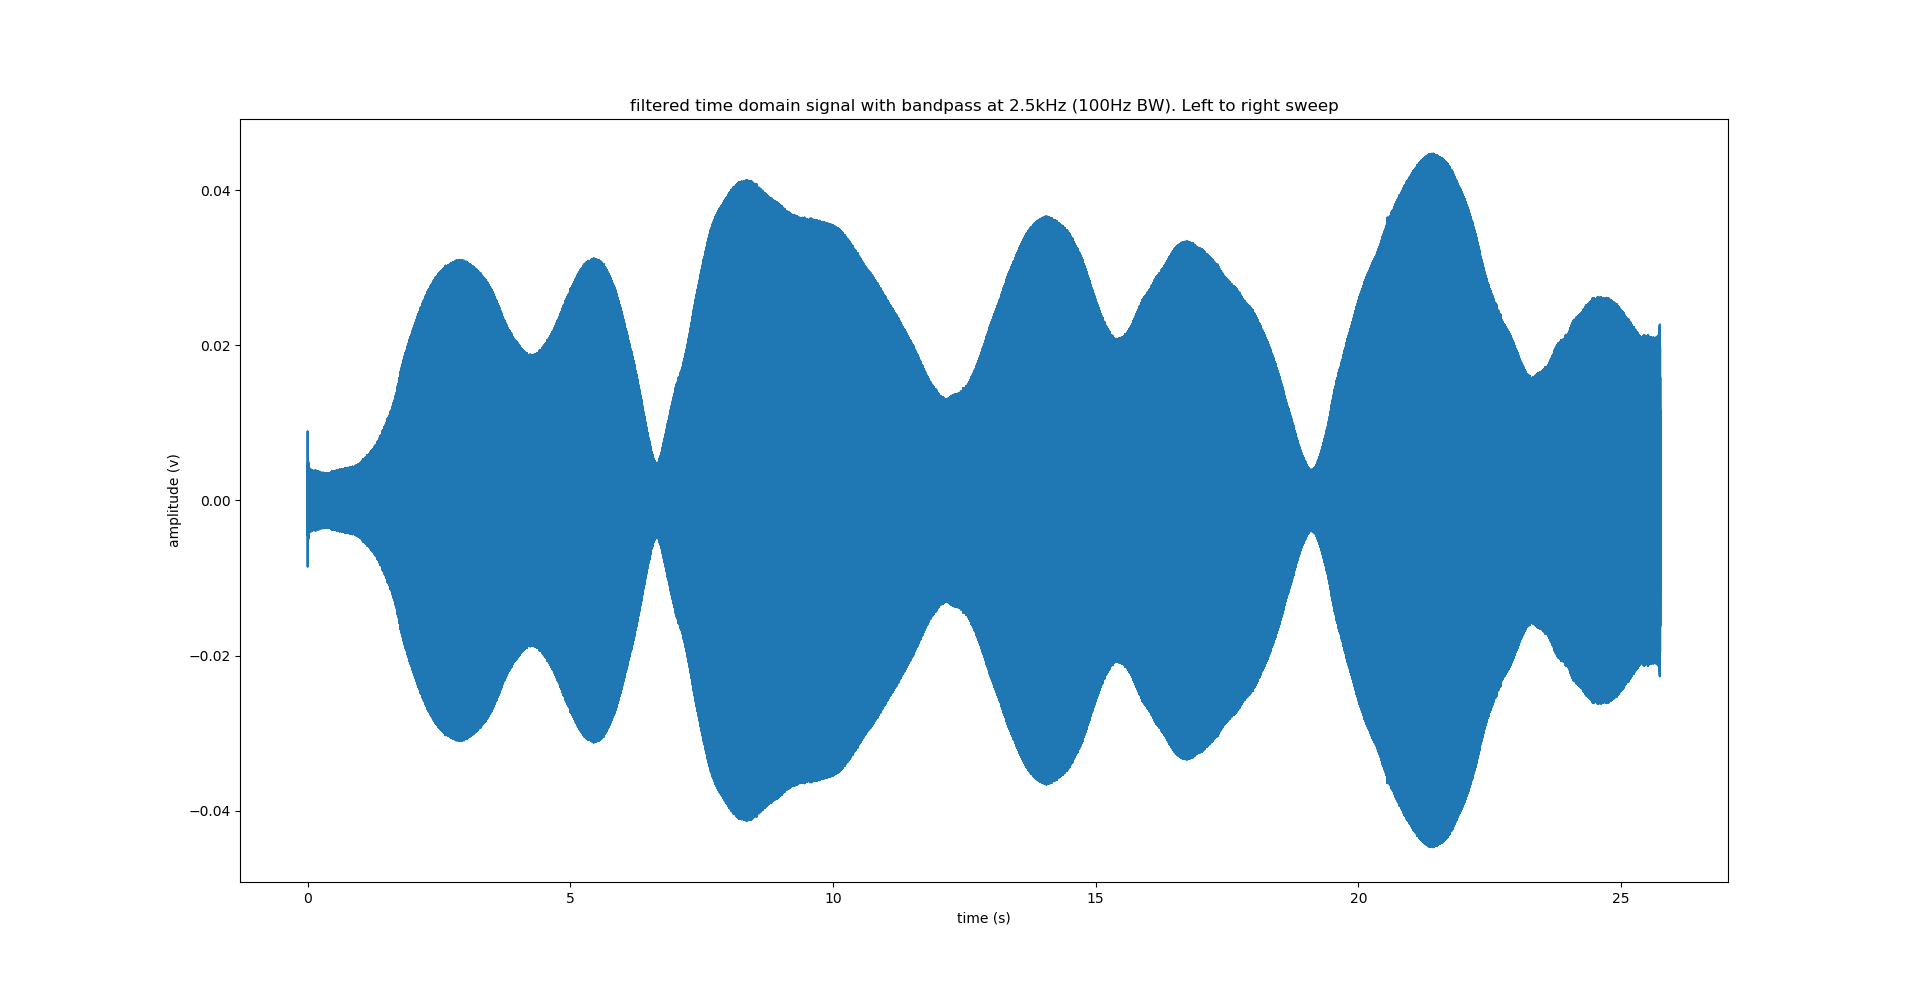
\includegraphics[width=\textwidth]{Figures/Testing/BeamSweep/Classical_speaker/2_5k_amp_sweep_spkr.png}
        \caption{Filtered 2.5kHz time domain signal emitted from a traditional speaker over beam sweep}
        \label{fig:spkr_sweep25k_amp}
    \end{minipage}\hfill
    \begin{minipage}{0.49\textwidth}
        \centering
        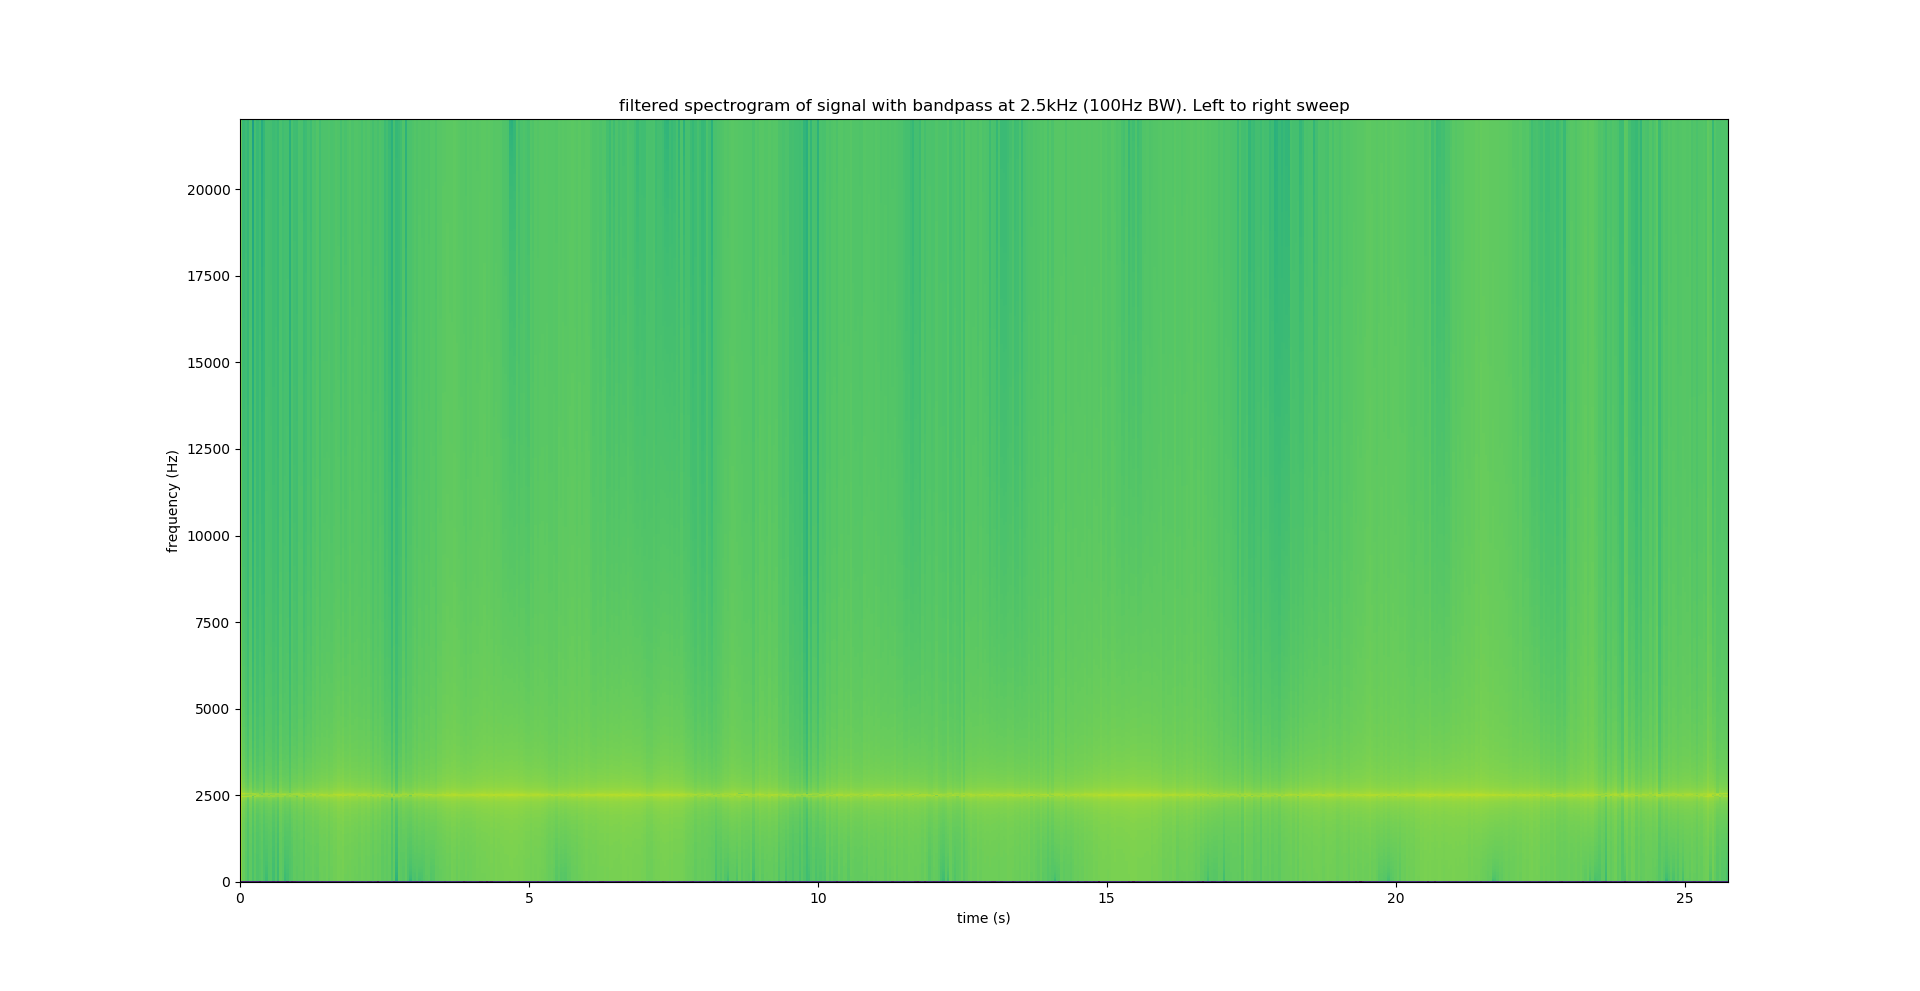
\includegraphics[width=\textwidth]{Figures/Testing/BeamSweep/Classical_speaker/2_5k_freq_sweep_spkr.png}
        \caption{Filtered 2.5kHz spectrum emitted from a traditional speaker over beam sweep}
        \label{fig:spkr_sweep25k_spectro}
    \end{minipage}
\end{figure}



\paragraph{5 kHz beam sweep results}

Figures \ref{fig:spkr_sweep5k_amp} and \ref{fig:spkr_sweep5k_spectro} show the time and frequency domain representations of the recorded beam sweep for a traditional loud speaker band-pass filtered at 5kHz. Figure \ref{fig:spkr_sweep5k_amp} demonstrates a lot more peaks and troughs over the entire beam sweep, oscillating between approximately $\pm$0.0004 V with the smallest troughs at around 9 and 20 seconds. The maximum peaks occur at approximately 14 and 22 seconds. The results represents a signal without significant directionality as there isn't a significant peak near the middle of the data. The spectrogram in figure \ref{fig:spkr_sweep5k_spectro} demonstrates what portion of the spectrum was used to create the time domain signal in figure \ref{fig:spkr_sweep5k_amp} but doesn't show significant variation in signal magnitude over the sweep, much like the 2.5kHz filtered result.
\begin{figure}[ht!]
    \centering
    \begin{minipage}{0.49\textwidth}
        \centering
        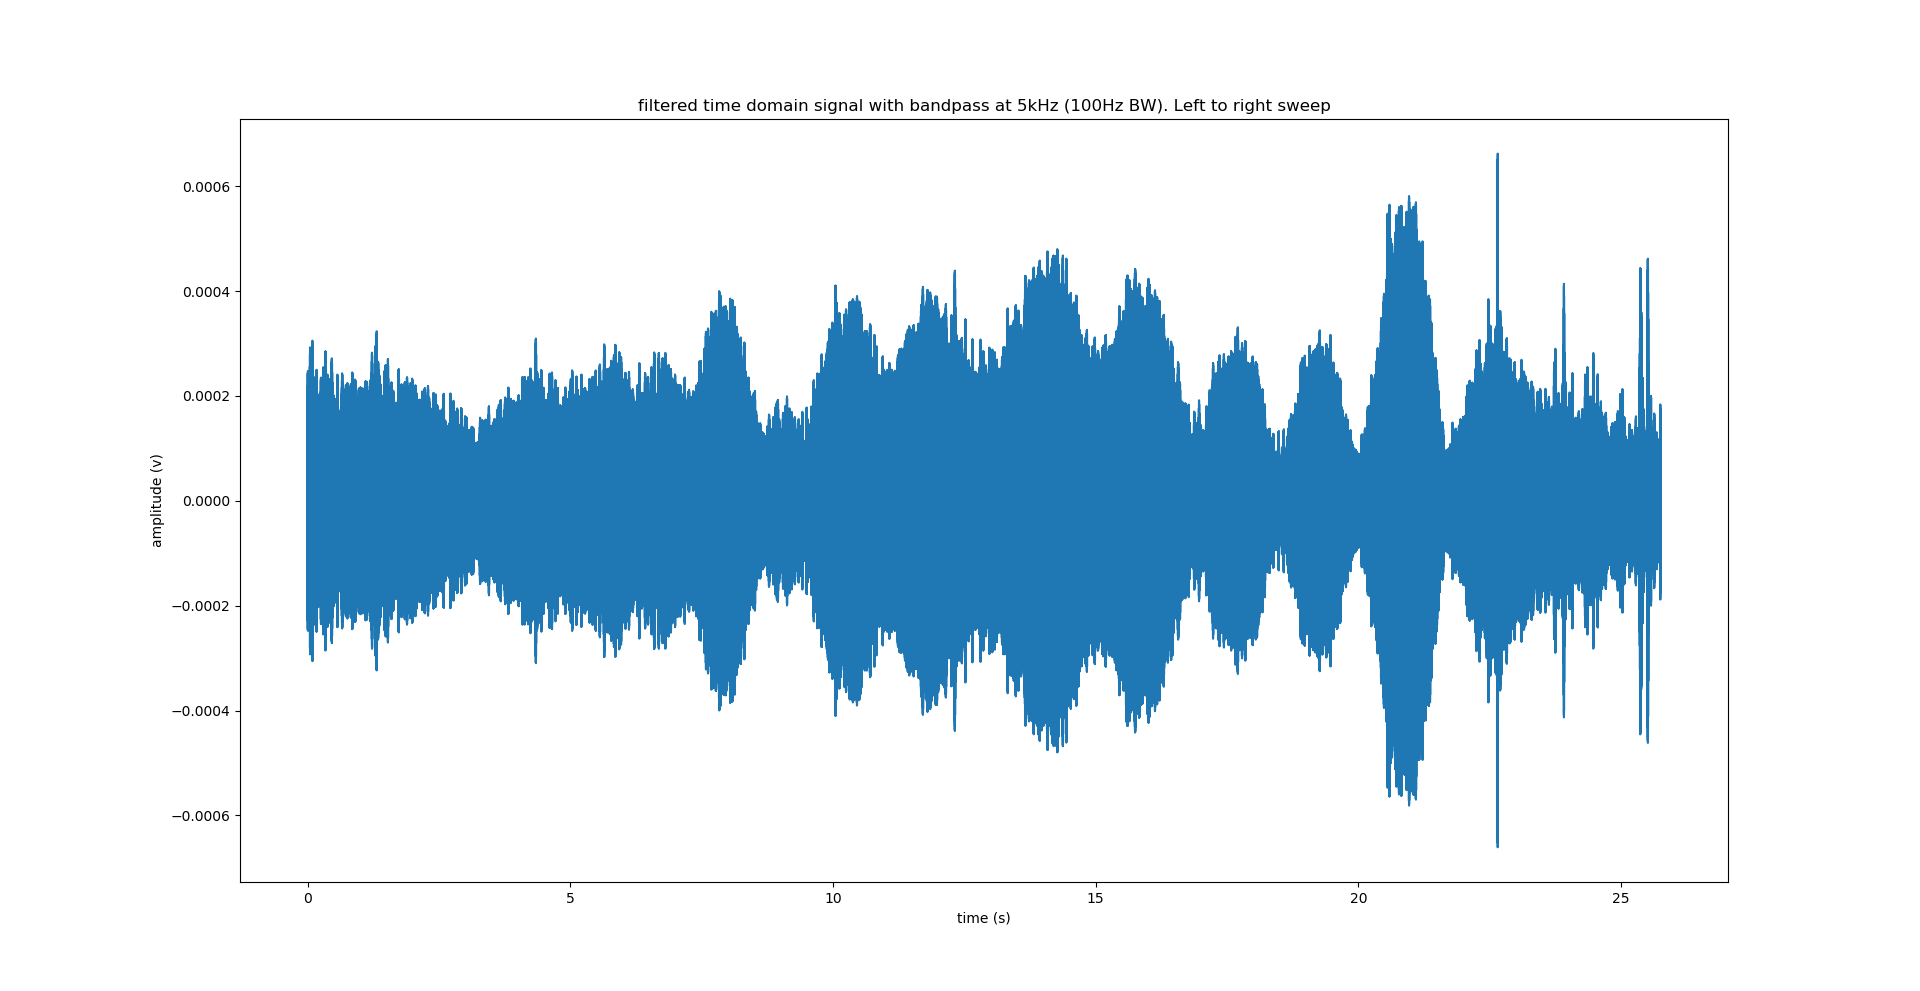
\includegraphics[width=\textwidth]{Figures/Testing/BeamSweep/Classical_speaker/5k_amp_sweep_spkr.png}
        \caption{Filtered 5kHz time domain signal emitted from a traditional speaker over beam sweep}
        \label{fig:spkr_sweep5k_amp}
    \end{minipage}\hfill
    \begin{minipage}{0.49\textwidth}
        \centering
        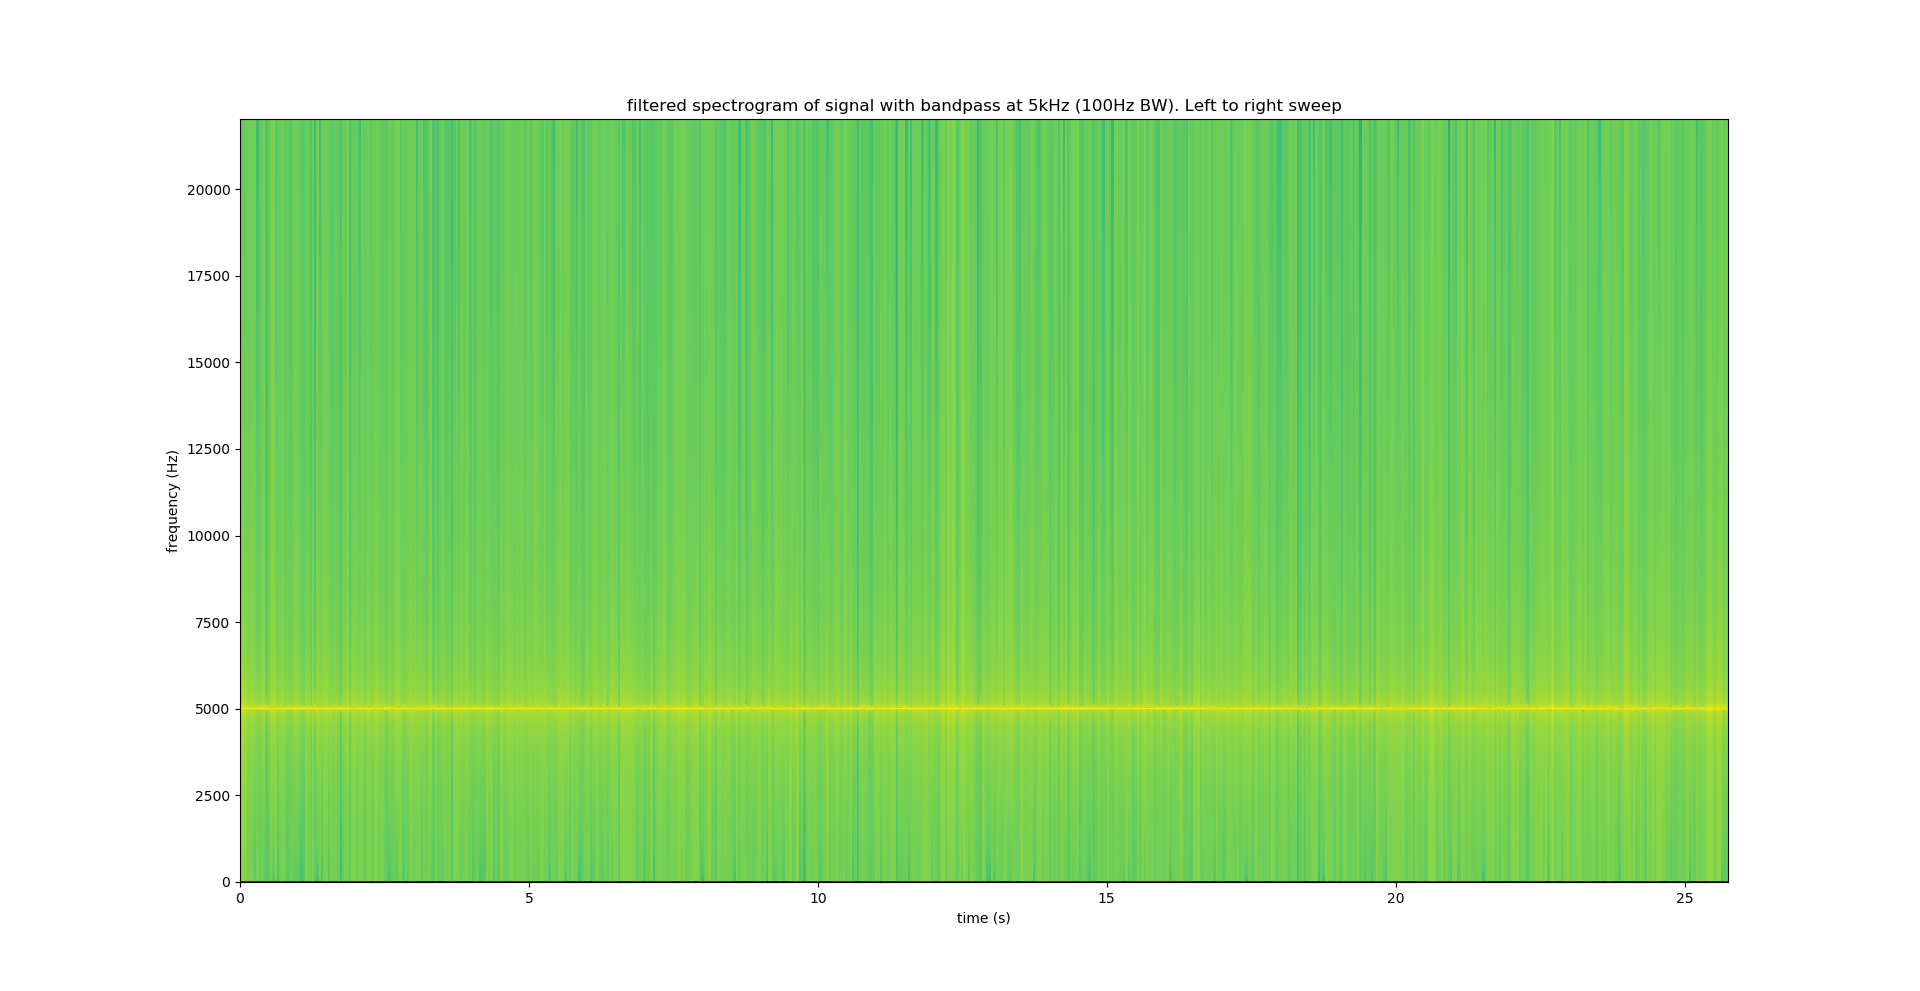
\includegraphics[width=\textwidth]{Figures/Testing/BeamSweep/Classical_speaker/5k_freq_sweep_spkr.png}
        \caption{Filtered 5kHz spectrum emitted from a traditional speaker over beam sweep}
        \label{fig:spkr_sweep5k_spectro}
    \end{minipage}
\end{figure}

\newpage
\paragraph{7.5 kHz beam sweep results}

Figures \ref{fig:spkr_sweep75k_amp} and \ref{fig:spkr_sweep75k_spectro} show the time and frequency domain representations of the recorded beam sweep for a traditional loud speaker band-pass filtered at 7.5kHz. Figure \ref{fig:spkr_sweep75k_amp} demonstrates few peaks over the entire beam sweep at relatively low magnitudes. The maximum peak should occur between 10 to 15 seconds if this were a directional beam but they instead appear before and after this region. The spectrogram in figure \ref{fig:spkr_sweep75k_spectro} demonstrates what portion of the spectrum was used to create the time domain signal in figure \ref{fig:spkr_sweep75k_amp} but doesn't show significant variation in signal magnitude over the sweep, much like the 2.5kHz filtered result.
\begin{figure}[ht!]
    \centering
    \begin{minipage}{0.49\textwidth}
        \centering
        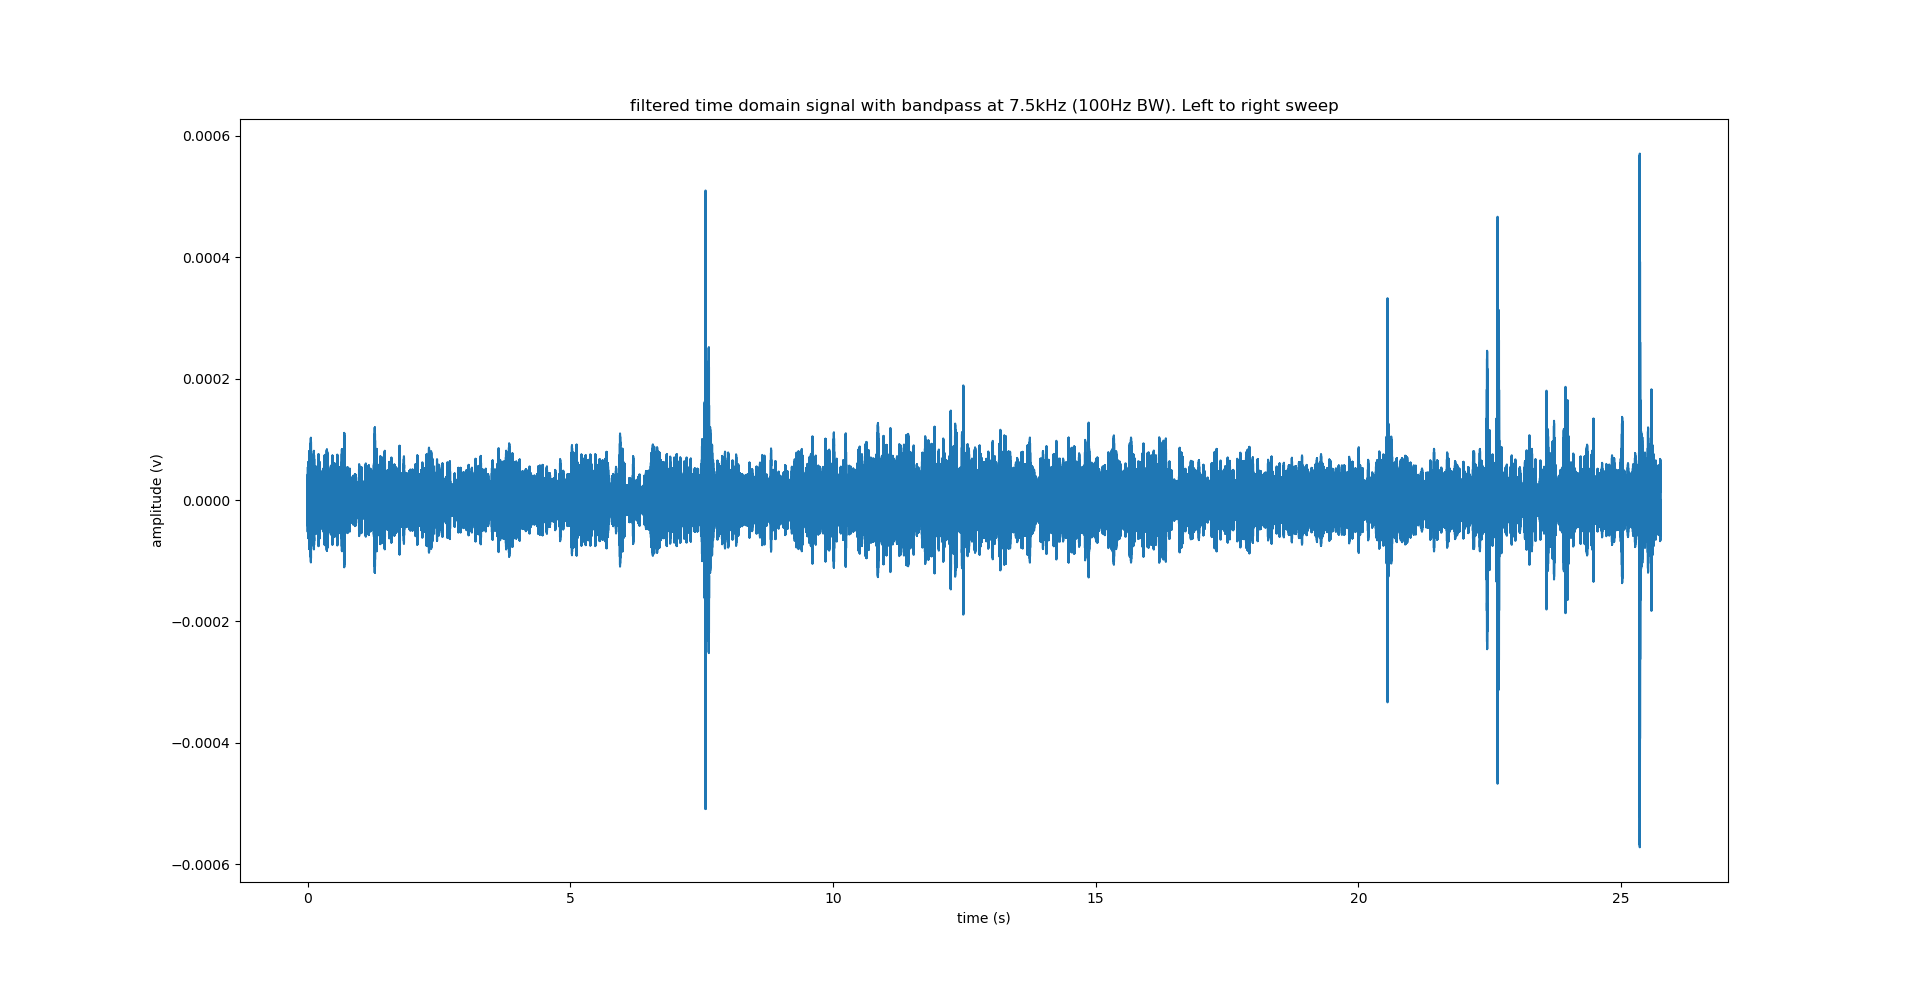
\includegraphics[width=\textwidth]{Figures/Testing/BeamSweep/Classical_speaker/7_5k_amp_sweep_spkr.png}
        \caption{Filtered 7.5kHz time domain signal emitted from a traditional speaker over beam sweep}
        \label{fig:spkr_sweep75k_amp}
    \end{minipage}\hfill
    \begin{minipage}{0.49\textwidth}
        \centering
        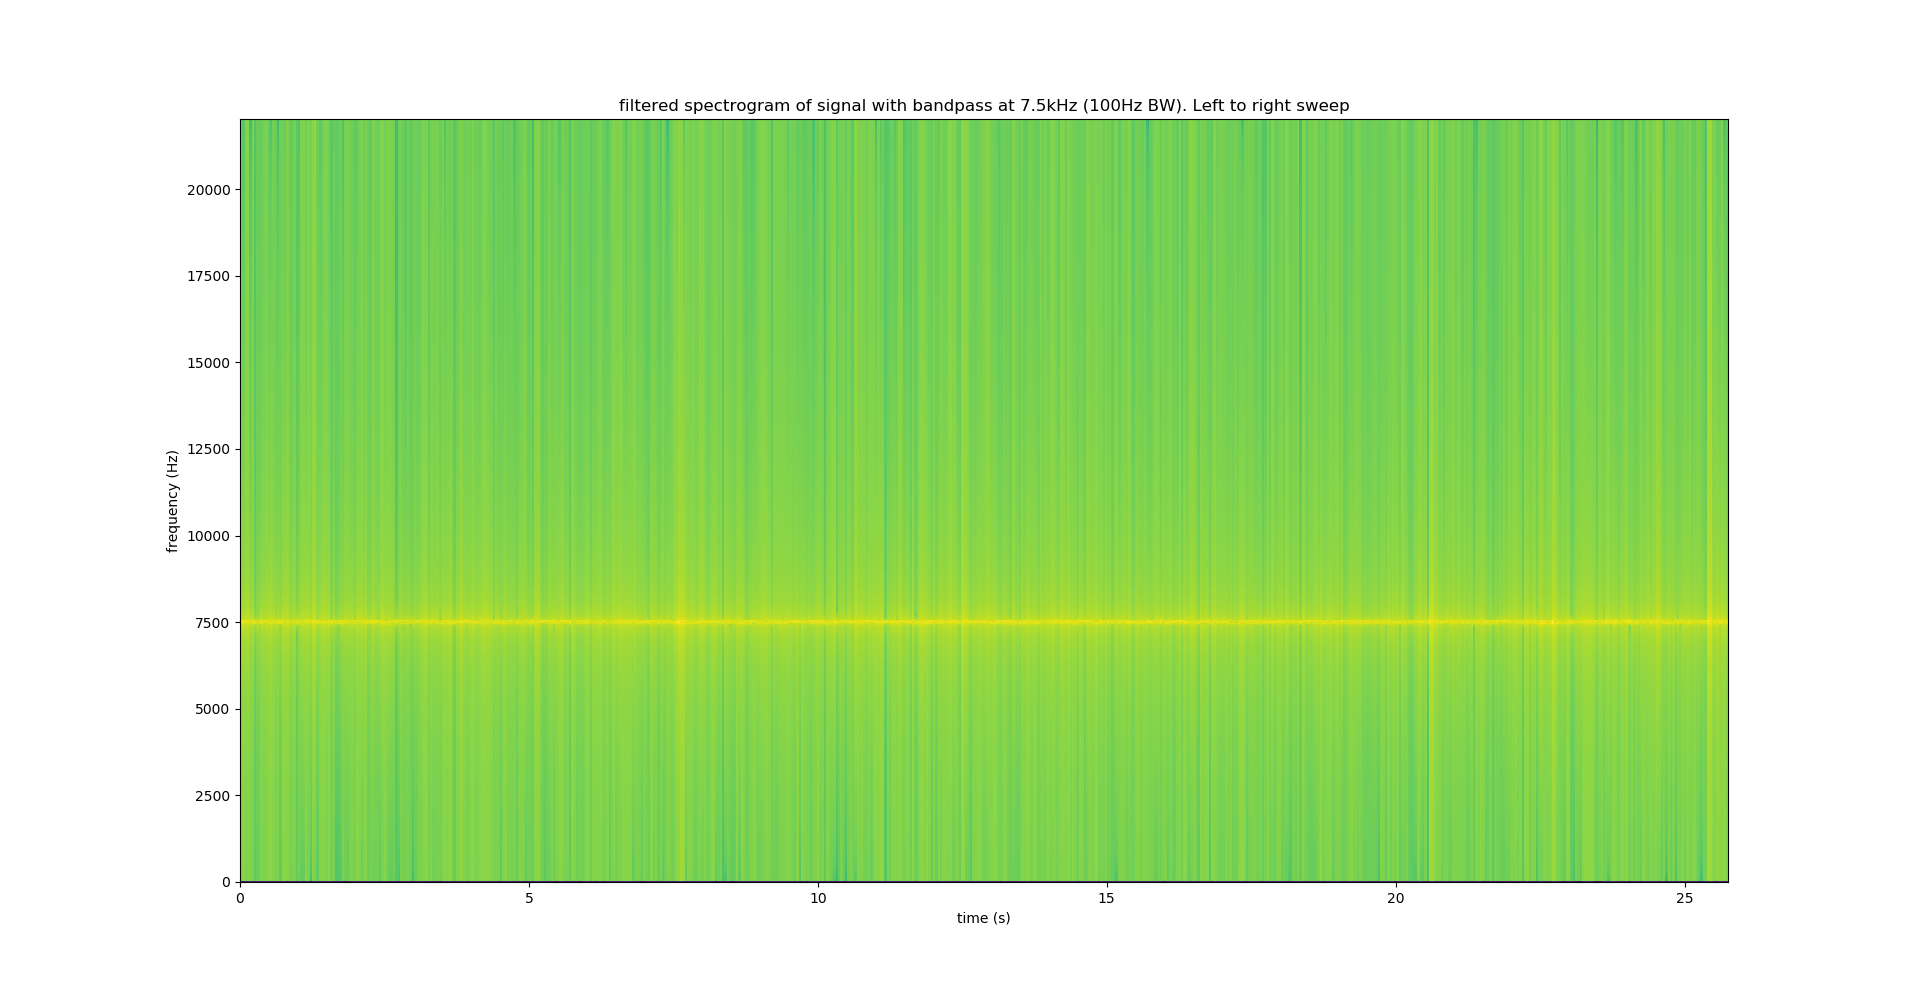
\includegraphics[width=\textwidth]{Figures/Testing/BeamSweep/Classical_speaker/7_5k_freq_sweep_spkr.png}
        \caption{Filtered 7.5kHz spectrum emitted from a traditional speaker over beam sweep}
        \label{fig:spkr_sweep75k_spectro}
    \end{minipage}
\end{figure}

\newpage

\subsubsection{Directivity of the directional audio system}
The results for the directional audio speaker are expected to show a significant spike in signal near the middle (10-15 seconds) as this is when the ultrasonic speaker's directional beam is in line with the microphone.
The unfiltered recording of the ultrasonic directional speaker beam sweep is analysed in figure \ref{fig:unfiltered_usonic_beamsweep} where the time and frequency domain representations of the signal are presented for the ultrasonic directional speaker beam sweep.
\begin{figure}[ht!]
    \centering
    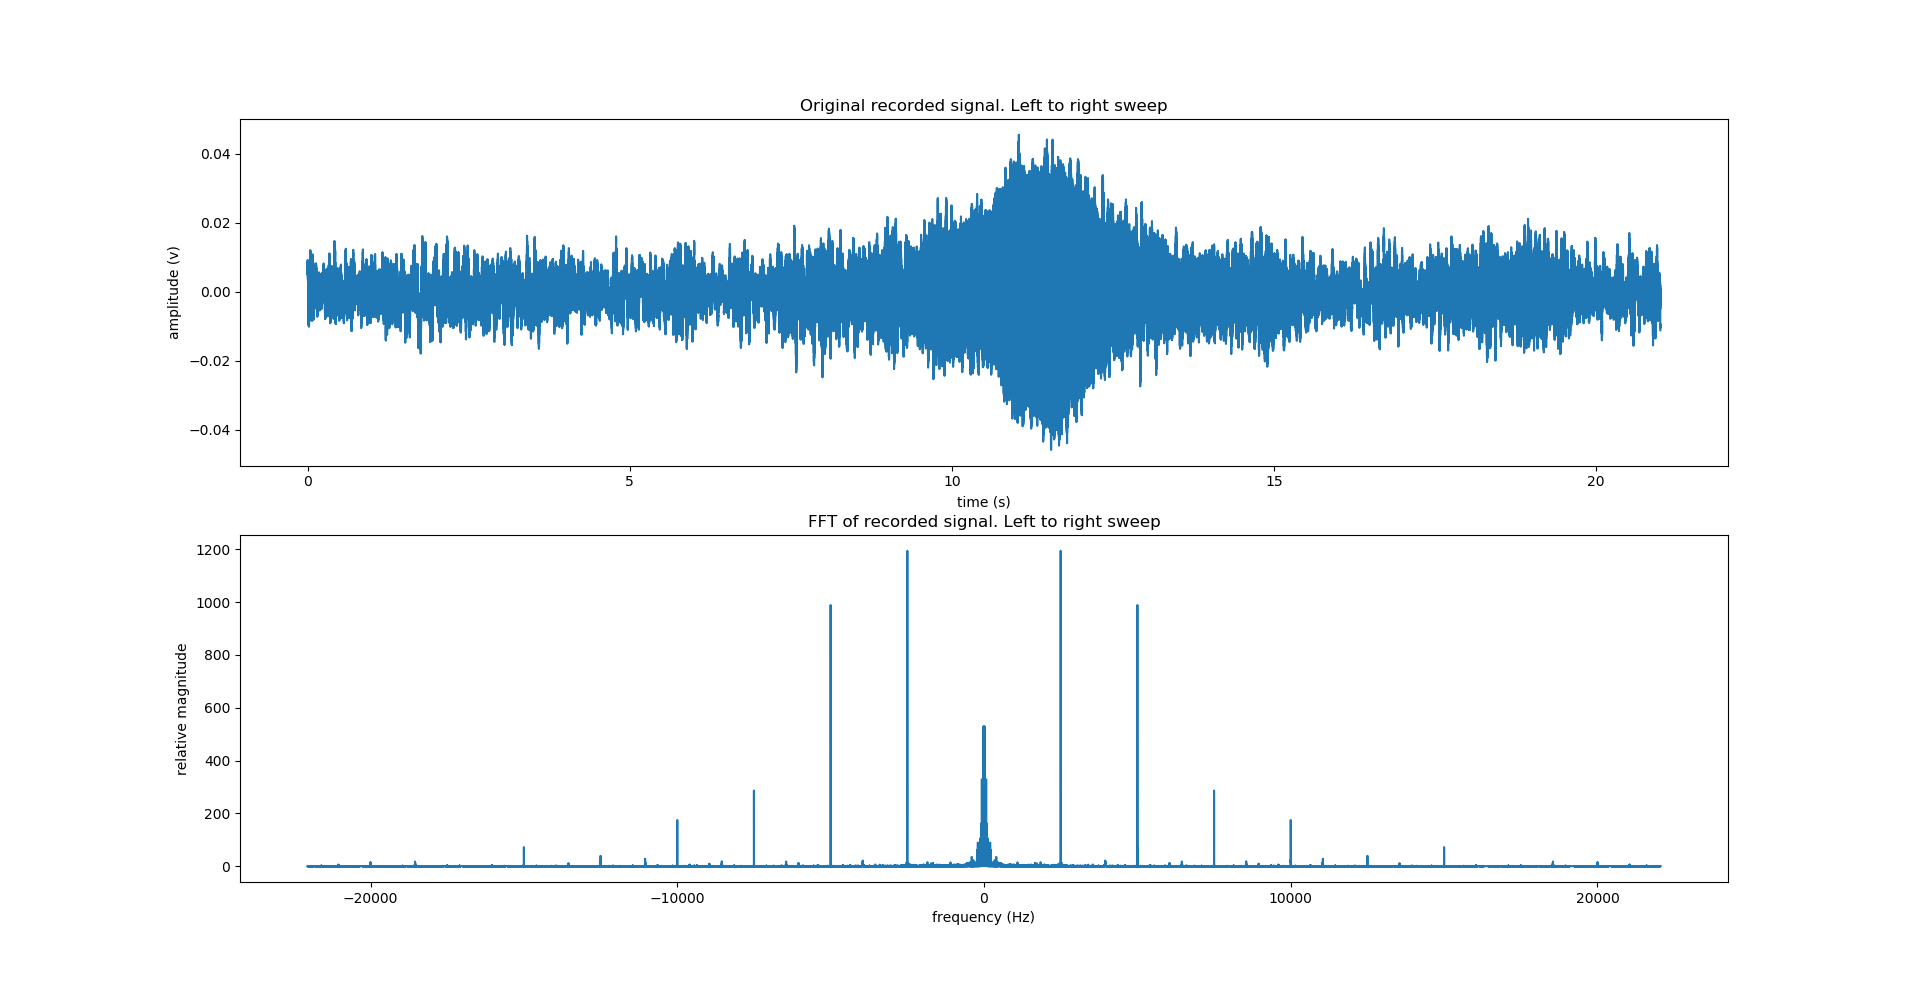
\includegraphics[width=0.9\textwidth]{Figures/Testing/BeamSweep/Ultrasonic_sqr_am/original_sig_fft_amp.png}
    \caption{Original beam sweep recording and FFT of all samples for ultrasonic directional speaker}
    \label{fig:unfiltered_usonic_beamsweep}
\end{figure}

\paragraph{Filtered 2.5 kHz beam sweep results}
Figures \ref{fig:usonic_sweep25k_amp} and \ref{fig:usonic_sweep25k_spectro} show the time and frequency domain representations of the recorded beam sweep for a ultrasonic directional speaker filtered to show the 2.5kHz fundamental tone. 
\begin{figure}[ht!]
    \centering
    \begin{minipage}{0.49\textwidth}
        \centering
        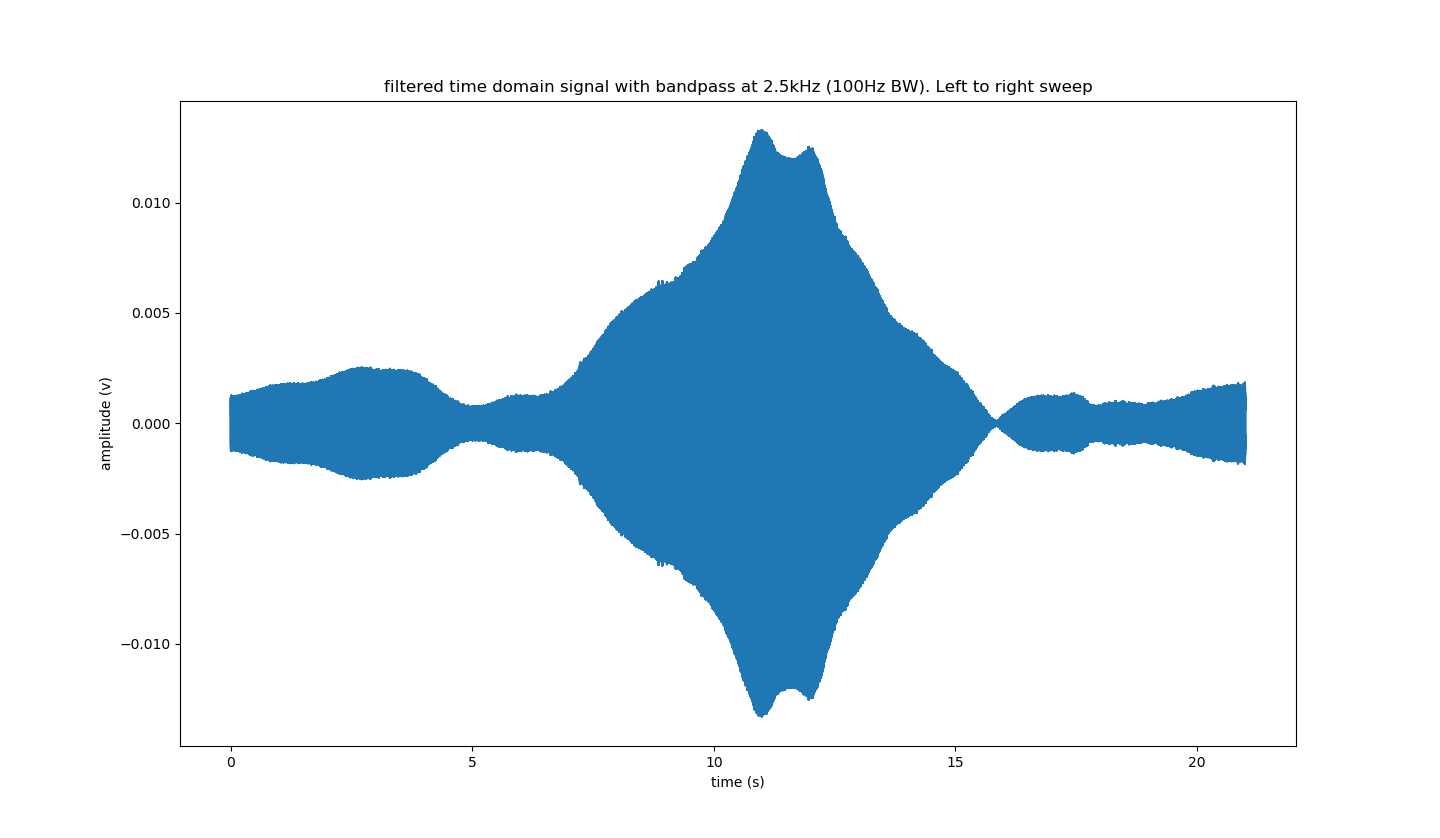
\includegraphics[width=\textwidth]{Figures/Testing/BeamSweep/Ultrasonic_sqr_am/2_5k_amp_sweep.png}
        \caption{Filtered 2.5kHz time domain signal emitted from a ultrasonic directional speaker over beam sweep}
        \label{fig:usonic_sweep25k_amp}
    \end{minipage}\hfill
    \begin{minipage}{0.49\textwidth}
        \centering
        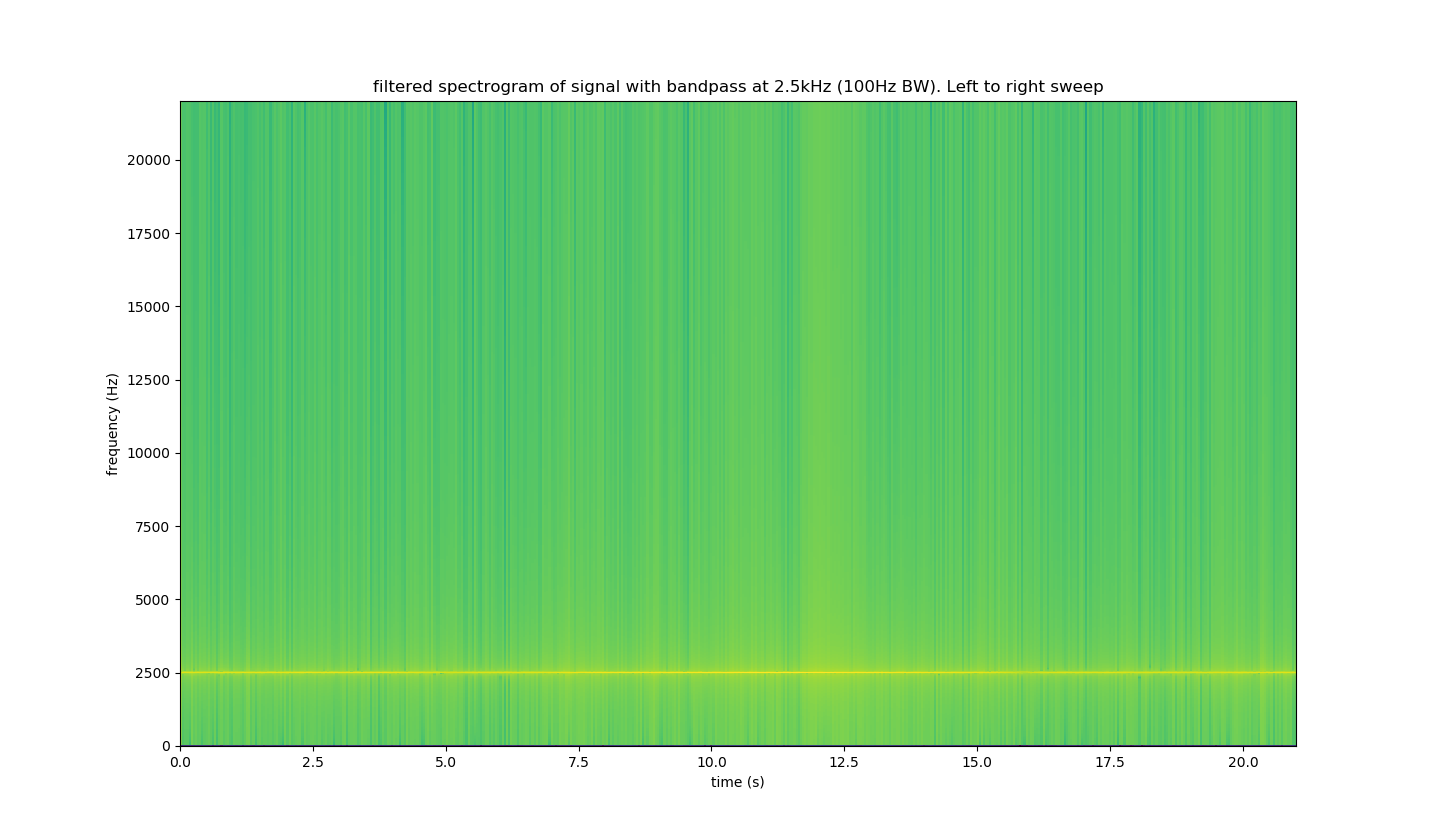
\includegraphics[width=\textwidth]{Figures/Testing/BeamSweep/Ultrasonic_sqr_am/2_5k_freq_sweep.png}
        \caption{Filtered 2.5kHz spectrum emitted from a ultrasonic directional speaker over beam sweep}
        \label{fig:usonic_sweep25k_spectro}
    \end{minipage}
\end{figure}
Figure \ref{fig:usonic_sweep25k_amp} shows a large spike in signal amplitude as the beam crosses the microphone with tapered edges on either side of this spike. Some minor fluctuations in the 2.5kHz signal are present before and after this spike and are likely from reflections of the beam off surfaces in the room. Note that there are two similarly sized maximum spikes at the apex of the sweep which may be the result of the beam reflecting off the wall behind the microphone, then passing over the microphone (causing the dip) and then reflecting once more. The spectrogram in figure \ref{fig:usonic_sweep25k_spectro} demonstrates what portion of the spectrum was used to create the time domain signal in figure \ref{fig:usonic_sweep25k_amp} and shows some increase in intensity as the recording reaches the 11 second mark.


\paragraph{Filtered 5 kHz beam sweep results}
Figures \ref{fig:usonic_sweep5k_amp} and \ref{fig:usonic_sweep5k_spectro} show the time and frequency domain representations of the recorded beam sweep for a ultrasonic directional speaker band-pass filtered to only show the 5kHz harmonic. 
\begin{figure}[ht!]
    \centering
    \begin{minipage}{0.49\textwidth}
        \centering
        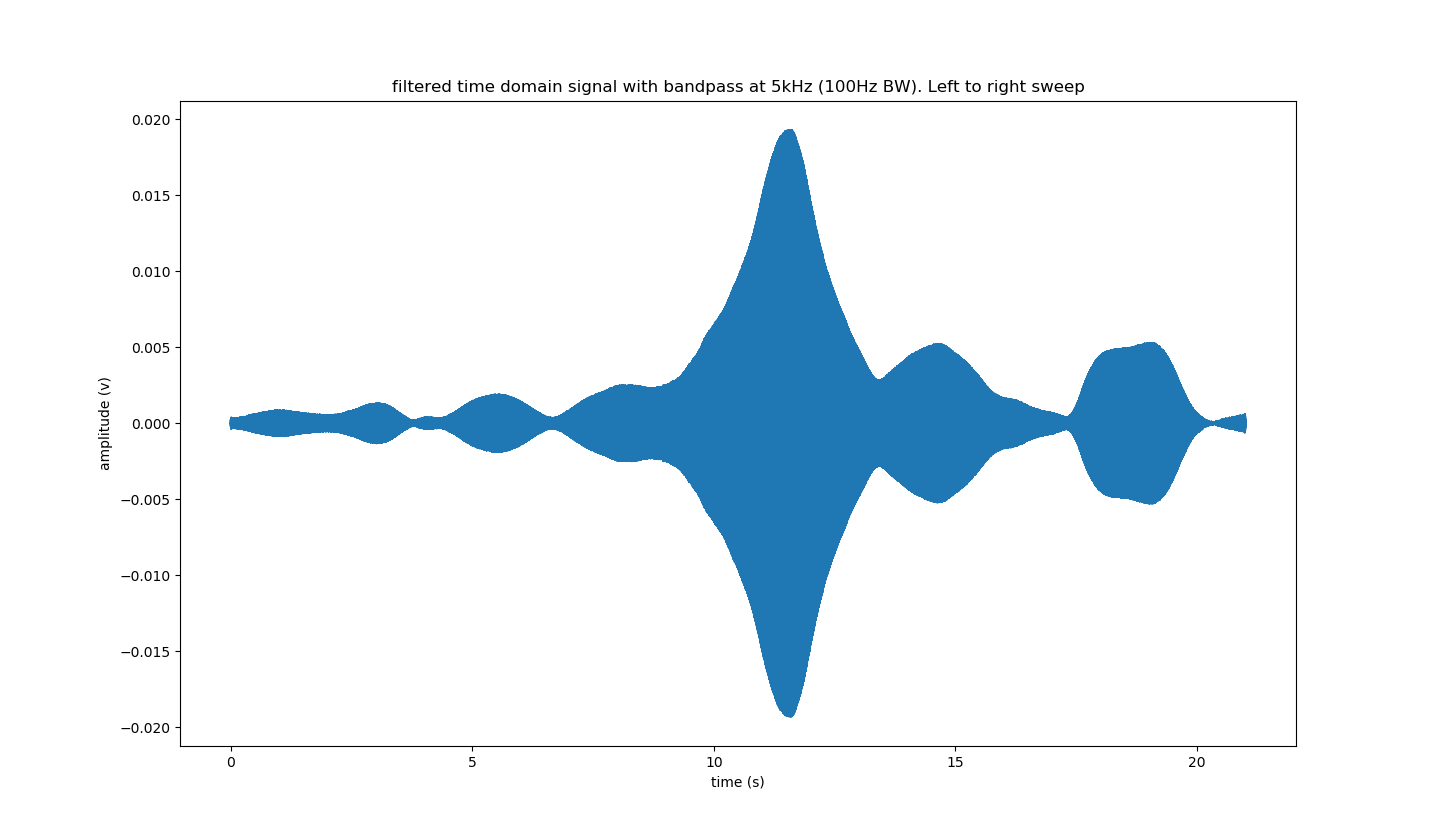
\includegraphics[width=\textwidth]{Figures/Testing/BeamSweep/Ultrasonic_sqr_am/5k_amp_sweep.png}
        \caption{Filtered 5kHz time domain signal emitted from a ultrasonic directional speaker over beam sweep}
        \label{fig:usonic_sweep5k_amp}
    \end{minipage}\hfill
    \begin{minipage}{0.49\textwidth}
        \centering
        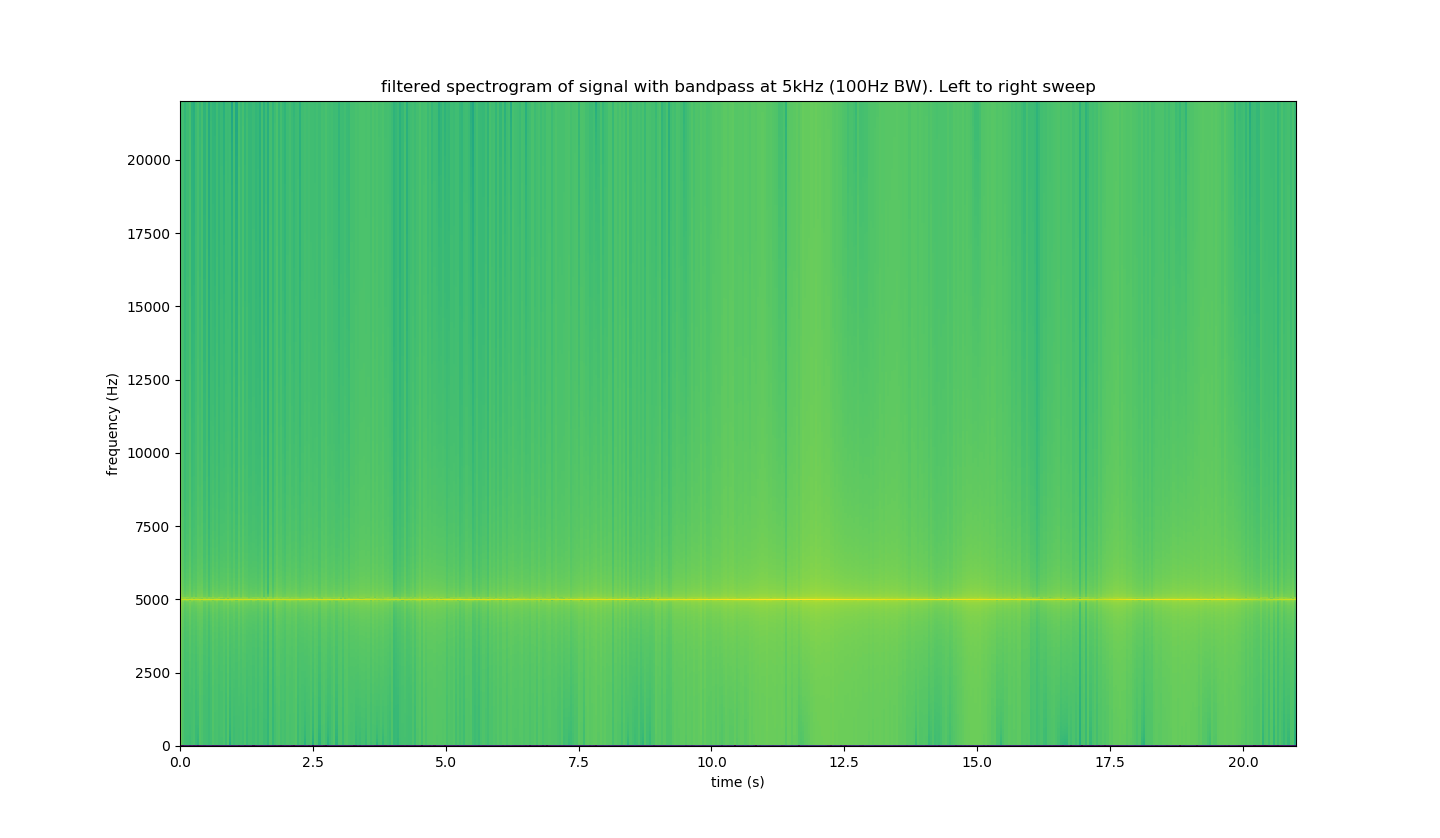
\includegraphics[width=\textwidth]{Figures/Testing/BeamSweep/Ultrasonic_sqr_am/5k_freq_sweep.png}
        \caption{Filtered 5kHz spectrum emitted from a ultrasonic directional speaker over beam sweep}
        \label{fig:usonic_sweep5k_spectro}
    \end{minipage}
\end{figure}
Figure \ref{fig:usonic_sweep5k_amp} shows a large spike in signal amplitude as the beam crosses the microphone with tapered edges on either side of this spike at 11 seconds. Before and after this main spike there exists some similarly shaped peaks in amplitude which could be the result of the side lobes of the beam as shown during the simulations in figure \ref{fig:sqr_elem_topBeam} and figure \ref{fig:sqr_elem_3Dbeam}. Alternatively it could be the result of reflections within the room causing pockets of constructive interference. Note however this is the first harmonic of the fundamental tone (2.5kHz) being produced which makes it somewhat undesirable as it isn't the original tone intended to be produced.
The magnitude of the main lobe's spike reaches near 0.04 V peak to peak, which is larger than the fundamental in figure \ref{fig:usonic_sweep25k_amp}. The shape of the main lobe is a lot narrower for the 5kHz harmonic than the 2.5kHz tone indicating that the first harmonic is a more directional beam than the fundamental while having larger side lobes than the 2.5kHz fundamental tone.
The spectrogram in figure \ref{fig:usonic_sweep5k_spectro} demonstrates what portion of the spectrum was used to create the time domain signal in figure \ref{fig:usonic_sweep5k_amp} and shows more intensity near the 11 second mark.

\paragraph{Filtered 7.5 kHz beam sweep results}
Figures \ref{fig:usonic_sweep75k_amp} and \ref{fig:usonic_sweep75k_spectro} show the time and frequency domain representations of the recorded beam sweep for a ultrasonic directional speaker band-pass filtered to only show the 7.5kHz harmonic. 
\begin{figure}[ht!]
    \centering
    \begin{minipage}{0.49\textwidth}
        \centering
        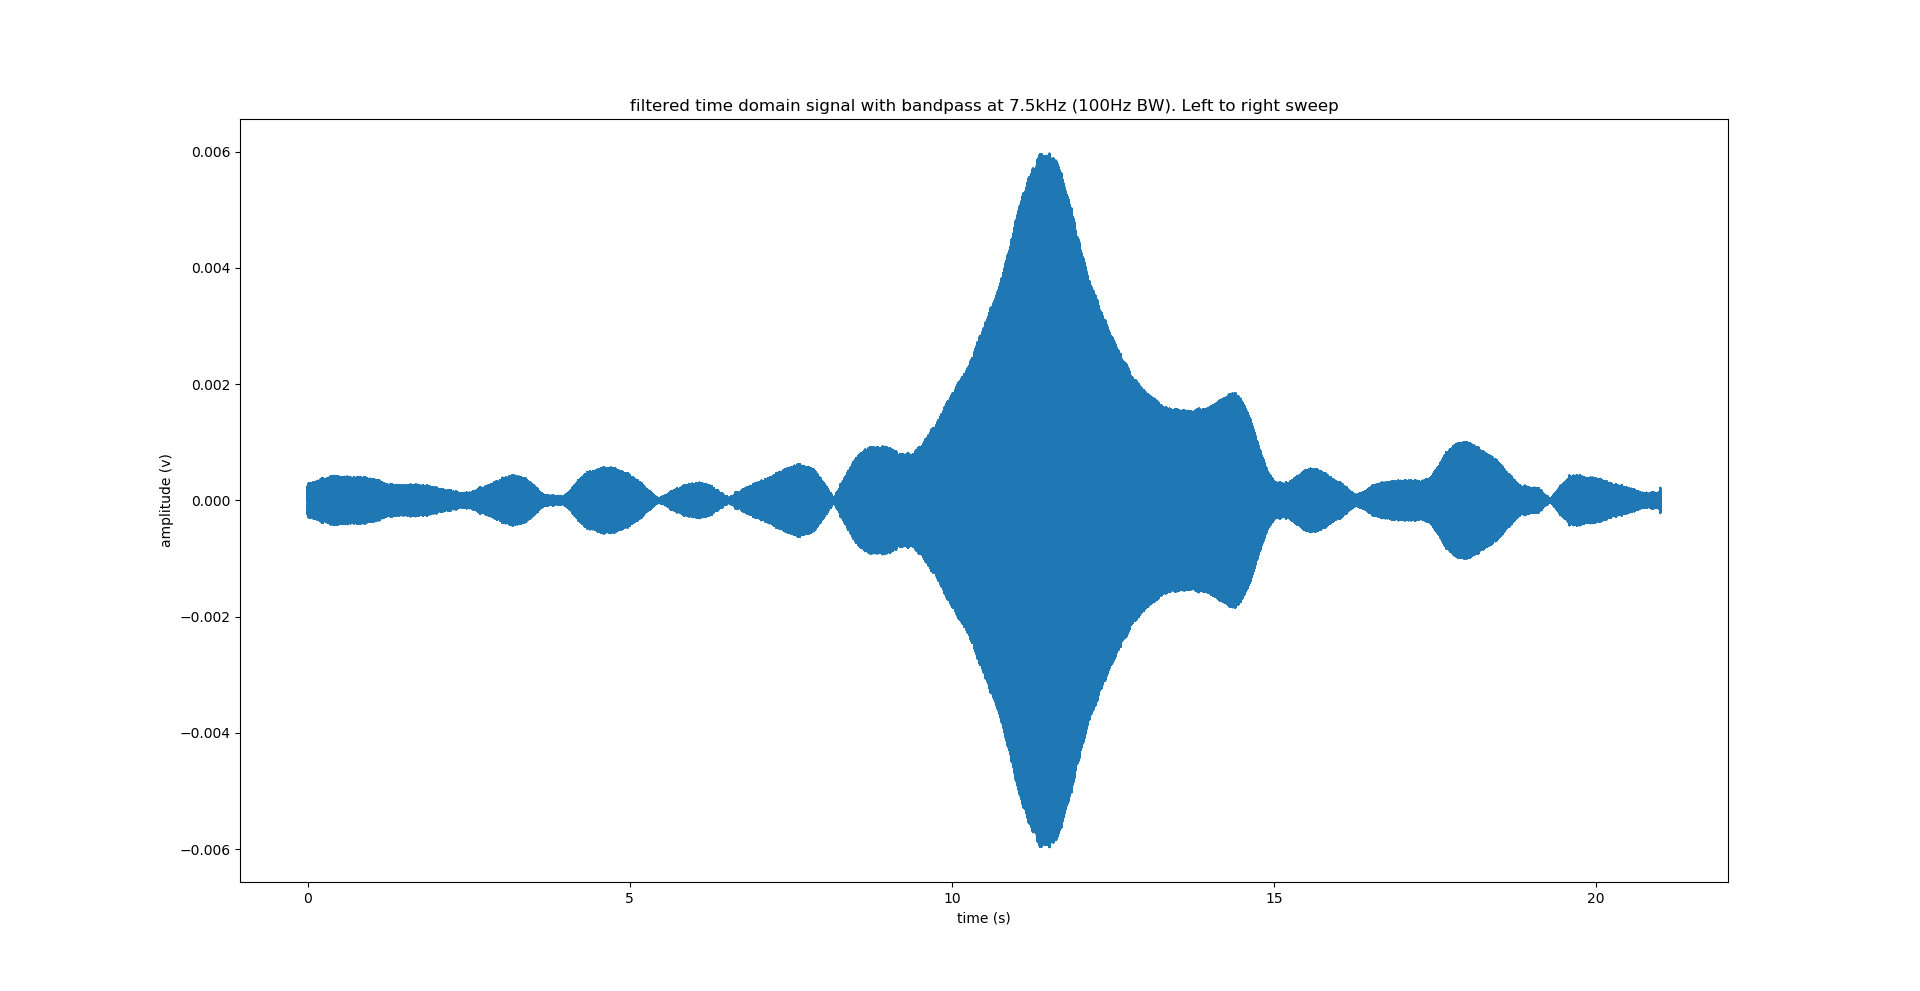
\includegraphics[width=\textwidth]{Figures/Testing/BeamSweep/Ultrasonic_sqr_am/7_5k_amp_sweep.png}
        \caption{Filtered 7.5kHz time domain signal emitted from a ultrasonic directional speaker over beam sweep}
        \label{fig:usonic_sweep75k_amp}
    \end{minipage}\hfill
    \begin{minipage}{0.49\textwidth}
        \centering
        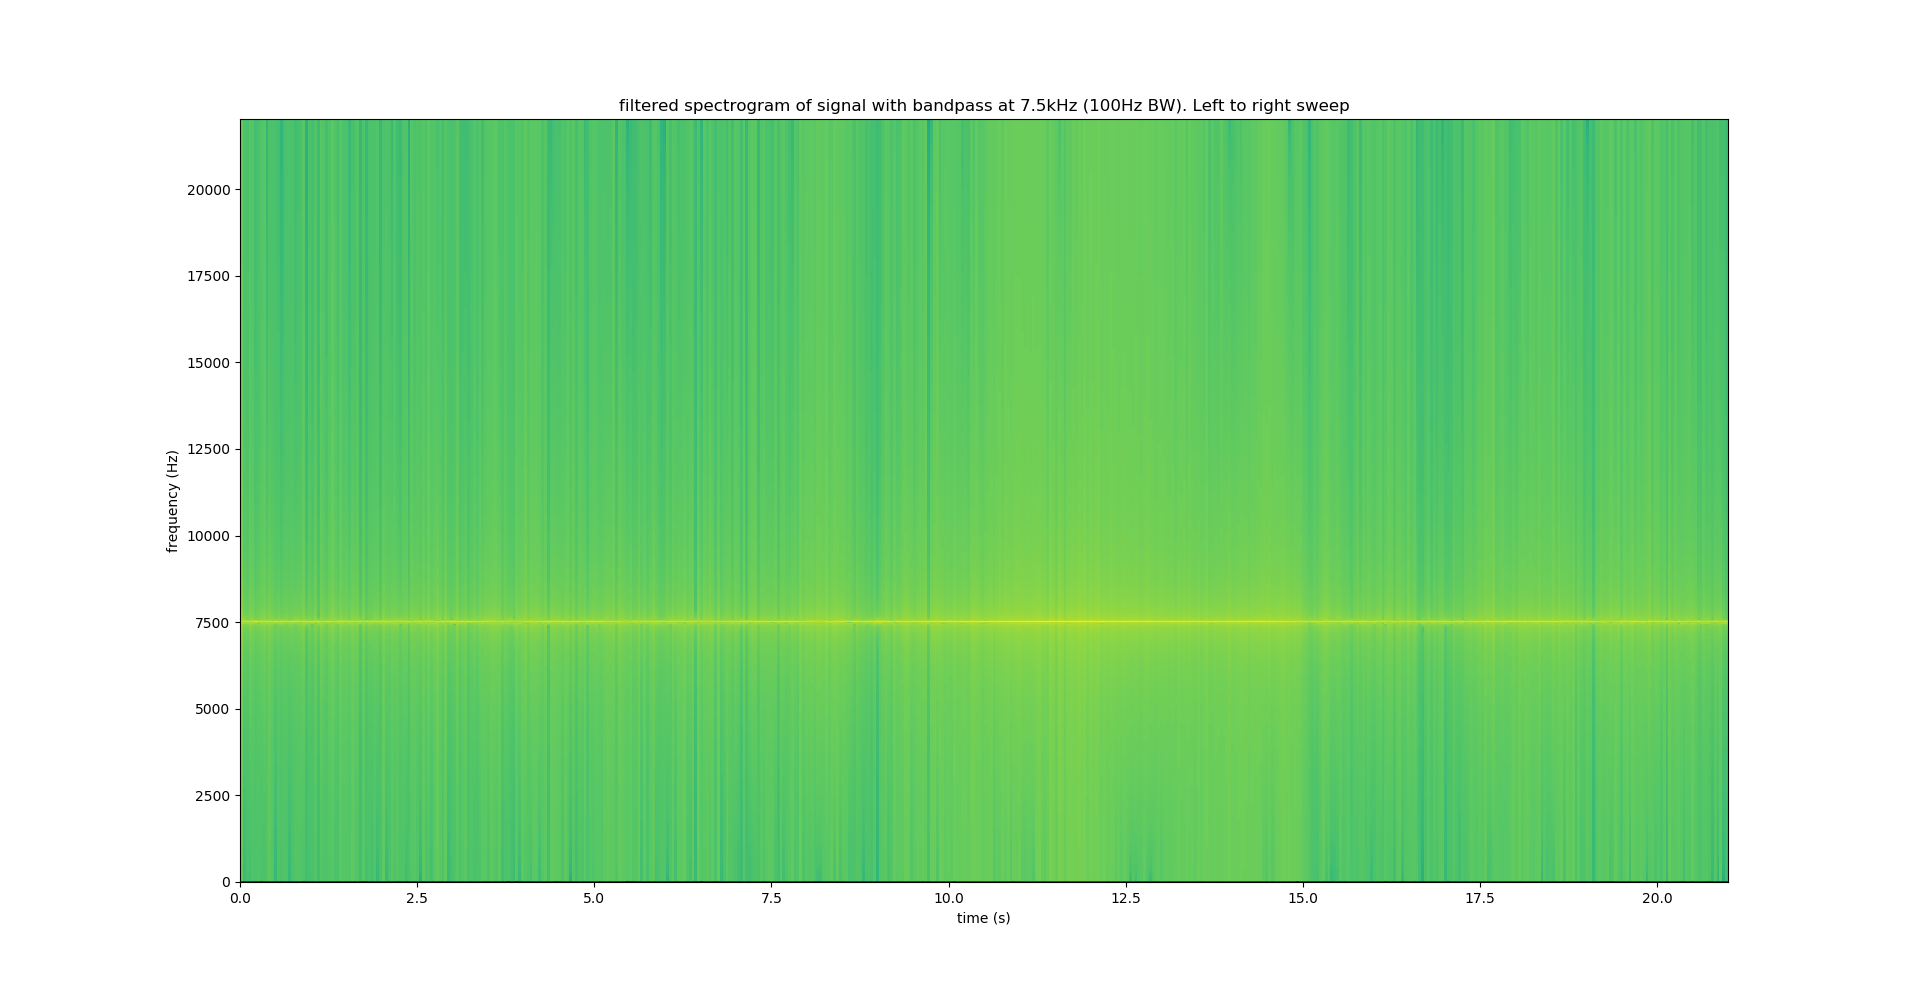
\includegraphics[width=\textwidth]{Figures/Testing/BeamSweep/Ultrasonic_sqr_am/7_5k_freq_sweep.png}
        \caption{Filtered 7.5kHz spectrum emitted from a ultrasonic directional speaker over beam sweep}
        \label{fig:usonic_sweep75k_spectro}
    \end{minipage}
\end{figure}
Figure \ref{fig:usonic_sweep75k_amp} shows a large spike in signal amplitude as the beam crosses the microphone with tapered edges on either side of this spike at 11 seconds. Before and after this main spike there exists some peaks in amplitude elsewhere in the beam sweep which are likely the result of reflections within the room causing pockets of constructive interference but could also indicate the presence of side lobes. Since this is the 2nd harmonic of the fundamental tone (2.5kHz) we would expect it to be of a significantly lower amplitude than the fundamental, which it does achieve with a peak to peak value of 0.012 V. This makes it still audible but at a lower intensity than the 1st harmonic and the fundamental (which are at similar intensities).
The shape of the main lobe is a lot narrower than the 2.5kHz result and has a similar sharpness to the 5kHz harmonic indicating that both the first and second harmonic are more directional beams than the fundamental tone. An asymmetry occurs for the 7.5kHz harmonic as the beam leaves the microphone. The intensity appears to taper off at a similar rate to its initial rise to the peak but then begins increasing again. This could be due to an asymmetric beam pattern or simply the corner of the room reflecting the directional beam back to the microphone and causing constructive interference.
The spectrogram in figure \ref{fig:usonic_sweep75k_spectro} demonstrates what portion of the spectrum was used to create the time domain signal in figure \ref{fig:usonic_sweep75k_amp} and shows more intensity as the recording approaches the 11 second mark, followed by a reduction in intensity.